%% (Master) Thesis template
% Template version used: v1.4
%
% Largely adapted from Adrian Nievergelt's template for the ADPS
% (lecture notes) project.



%% We use the memoir class because it offers a many easy to use features.
\documentclass[11pt,a4paper,titlepage]{memoir}

%% Packages
%% ========

% for revision
\usepackage{float}
%% LaTeX Font encoding -- DO NOT CHANGE
\usepackage[OT1]{fontenc}

%% Babel provides support for languages.  'english' uses British
%% English hyphenation and text snippets like "Figure" and
%% "Theorem". Use the option 'ngerman' if your document is in German.
%% Use 'american' for American English.  Note that if you change this,
%% the next LaTeX run may show spurious errors.  Simply run it again.
%% If they persist, remove the .aux file and try again.
\usepackage[american]{babel}

%% Input encoding 'utf8'. In some cases you might need 'utf8x' for
%% extra symbols. Not all editors, especially on Windows, are UTF-8
%% capable, so you may want to use 'latin1' instead.
\usepackage[utf8]{inputenc}

%% This changes default fonts for both text and math mode to use Herman Zapfs
%% excellent Palatino font.  Do not change this.
\usepackage[sc]{mathpazo}

%% The AMS-LaTeX extensions for mathematical typesetting.  Do not
%% remove.
\usepackage{amsmath,amssymb,amsfonts,mathrsfs}

%% NTheorem is a reimplementation of the AMS Theorem package. This
%% will allow us to typeset theorems like examples, proofs and
%% similar.  Do not remove.
%% NOTE: Must be loaded AFTER amsmath, or the \qed placement will
%% break
\usepackage[amsmath,thmmarks]{ntheorem}

%% LaTeX' own graphics handling
\usepackage{graphicx}

%% We unfortunately need this for the Rules chapter.  Remove it
%% afterwards; or at least NEVER use its underlining features.
\usepackage{soul}

%% This allows you to add .pdf files. It is used to add the
%% declaration of originality.
\usepackage{pdfpages}

%% Some more packages that you may want to use.  Have a look at the
%% file, and consult the package docs for each.
%% See the TeXed file for more explanations

%% [OPT] Multi-rowed cells in tabulars
%\usepackage{multirow}

%% [REC] Intelligent cross reference package. This allows for nice
%% combined references that include the reference and a hint to where
%% to look for it.
\usepackage{varioref}

%% [OPT] Easily changeable quotes with \enquote{Text}
%\usepackage[german=swiss]{csquotes}

%% [REC] Format dates and time depending on locale
\usepackage{datetime}

%% [OPT] Provides a \cancel{} command to stroke through mathematics.
%\usepackage{cancel}

%% [NEED] This allows for additional typesetting tools in mathmode.
%% See its excellent documentation.
\usepackage{mathtools}

%% [ADV] Conditional commands
%\usepackage{ifthen}

%% [OPT] Manual large braces or other delimiters.
%\usepackage{bigdelim, bigstrut}

%% [REC] Alternate vector arrows. Use the command \vv{} to get scaled
%% vector arrows.
\usepackage[h]{esvect}

%% [NEED] Some extensions to tabulars and array environments.
\usepackage{array}

%% [OPT] Postscript support via pstricks graphics package. Very
%% diverse applications.
%\usepackage{pstricks,pst-all}

%% [?] This seems to allow us to define some additional counters.
%\usepackage{etex}

%% [ADV] XY-Pic to typeset some matrix-style graphics
%\usepackage[all]{xy}

%% [OPT] This is needed to generate an index at the end of the
%% document.
%\usepackage{makeidx}

%% [OPT] Fancy package for source code listings.  The template text
%% needs it for some LaTeX snippets; remove/adapt the \lstset when you
%% remove the template content.
\usepackage{listings}
\lstset{language=TeX,basicstyle={\normalfont\ttfamily}}

%% [REC] Fancy character protrusion.  Must be loaded after all fonts.
\usepackage[activate]{pdfcprot}

%% [REC] Nicer tables.  Read the excellent documentation.
\usepackage{booktabs}


%% Our layout configuration.  DO NOT CHANGE.
%% Memoir layout setup

%% NOTE: You are strongly advised not to change any of them unless you
%% know what you are doing.  These settings strongly interact in the
%% final look of the document.

% Dependencies

% Turn extra space before chapter headings off.
\setlength{\beforechapskip}{0pt}

\nonzeroparskip
\parindent=0pt
\defaultlists

% Chapter style redefinition
\makeatletter

\if@twoside
  \pagestyle{Ruled}
  \copypagestyle{chapter}{Ruled}
\else
  \pagestyle{ruled}
  \copypagestyle{chapter}{ruled}
\fi
\makeoddhead{chapter}{}{}{}
\makeevenhead{chapter}{}{}{}
\makeheadrule{chapter}{\textwidth}{0pt}
\copypagestyle{abstract}{empty}

\makechapterstyle{bianchimod}{%
  \chapterstyle{default}
  \renewcommand*{\chapnamefont}{\normalfont\Large\sffamily}
  \renewcommand*{\chapnumfont}{\normalfont\Large\sffamily}
  \renewcommand*{\printchaptername}{%
    \chapnamefont\centering\@chapapp}
  \renewcommand*{\printchapternum}{\chapnumfont {\thechapter}}
  \renewcommand*{\chaptitlefont}{\normalfont\huge\sffamily}
  \renewcommand*{\printchaptertitle}[1]{%
    \hrule\vskip\onelineskip \centering \chaptitlefont\textbf{\vphantom{gyM}##1}\par}
  \renewcommand*{\afterchaptertitle}{\vskip\onelineskip \hrule\vskip
    \afterchapskip}
  \renewcommand*{\printchapternonum}{%
    \vphantom{\chapnumfont {9}}\afterchapternum}}

% Use the newly defined style
\chapterstyle{bianchimod}

\setsecheadstyle{\Large\bfseries\sffamily}
\setsubsecheadstyle{\large\bfseries\sffamily}
\setsubsubsecheadstyle{\bfseries\sffamily}
\setparaheadstyle{\normalsize\bfseries\sffamily}
\setsubparaheadstyle{\normalsize\itshape\sffamily}
\setsubparaindent{0pt}

% Set captions to a more separated style for clearness
\captionnamefont{\sffamily\bfseries\footnotesize}
\captiontitlefont{\sffamily\footnotesize}
\setlength{\intextsep}{16pt}
\setlength{\belowcaptionskip}{1pt}

% Set section and TOC numbering depth to subsection
\setsecnumdepth{subsection}
\settocdepth{subsection}
%%begin novalidate
%% Titlepage adjustments
\pretitle{\vspace{0pt plus 0.7fill}\begin{center}\HUGE\sffamily\bfseries}
\posttitle{\end{center}\par}
\preauthor{\par\begin{center}\let\and\\\Large\sffamily}
\postauthor{\end{center}}
\predate{\par\begin{center}\Large\sffamily}
\postdate{\end{center}}
%%end novalidate
\def\@advisors{}
\newcommand{\advisors}[1]{\def\@advisors{#1}}
\def\@department{}
\newcommand{\department}[1]{\def\@department{#1}}
\def\@thesistype{}
\newcommand{\thesistype}[1]{\def\@thesistype{#1}}

%\renewcommand{\maketitlehooka}{\noindent\ETHlogo[2in]}

\renewcommand{\maketitlehookb}{\vspace{1in}%
  \par\begin{center}\Large\sffamily\@thesistype\end{center}}

\renewcommand{\maketitlehookd}{%
  \vfill\par
  \begin{flushright}
    \sffamily
    \@advisors\par
    \@department, Idaho State University
  \end{flushright}
}

\checkandfixthelayout

\setlength{\droptitle}{-48pt}

\makeatother

% This defines how theorems should look. Best leave as is.
\theoremstyle{plain}
\setlength\theorempostskipamount{0pt}

%%% Local Variables:
%%% mode: latex
%%% TeX-master: "thesis"
%%% End:


%% Theorem environments.  You will have to adapt this for a German
%% thesis.
%% Theorem-like environments

%% This can be changed according to language. You can comment out the ones you
%% don't need.

\numberwithin{equation}{chapter}

%% German theorems
%\newtheorem{satz}{Satz}[chapter]
%\newtheorem{beispiel}[satz]{Beispiel}
%\newtheorem{bemerkung}[satz]{Bemerkung}
%\newtheorem{korrolar}[satz]{Korrolar}
%\newtheorem{definition}[satz]{Definition}
%\newtheorem{lemma}[satz]{Lemma}
%\newtheorem{proposition}[satz]{Proposition}

%% English variants
\newtheorem{theorem}{Theorem}[chapter]
\newtheorem{example}[theorem]{Example}
\newtheorem{remark}[theorem]{Remark}
\newtheorem{corollary}[theorem]{Corollary}
\newtheorem{definition}[theorem]{Definition}
\newtheorem{lemma}[theorem]{Lemma}
\newtheorem{proposition}[theorem]{Proposition}

%% Proof environment with a small square as a "qed" symbol
\theoremstyle{nonumberplain}
\theorembodyfont{\normalfont}
\theoremsymbol{\ensuremath{\square}}
\newtheorem{proof}{Proof}
%\newtheorem{beweis}{Beweis}


%% Helpful macros.
%% Custom commands
%% ===============

%% Special characters for number sets, e.g. real or complex numbers.
\newcommand{\C}{\mathbb{C}}
\newcommand{\K}{\mathbb{K}}
\newcommand{\N}{\mathbb{N}}
\newcommand{\Q}{\mathbb{Q}}
\newcommand{\R}{\mathbb{R}}
\newcommand{\Z}{\mathbb{Z}}
\newcommand{\X}{\mathbb{X}}

%% Fixed/scaling delimiter examples (see mathtools documentation)
\DeclarePairedDelimiter\abs{\lvert}{\rvert}
\DeclarePairedDelimiter\norm{\lVert}{\rVert}

%% Use the alternative epsilon per default and define the old one as \oldepsilon
\let\oldepsilon\epsilon
\renewcommand{\epsilon}{\ensuremath\varepsilon}

%% Also set the alternate phi as default.
\let\oldphi\phi
\renewcommand{\phi}{\ensuremath{\varphi}}

\usepackage{multirow,bm,siunitx}
\usepackage{longtable,booktabs}
\usepackage{siunitx}
\usepackage{pifont}% http://ctan.org/pkg/pifont
 \usepackage{relsize}
\sisetup{table-number-alignment=center, exponent-product=\cdot}

%% Make document internal hyperlinks wherever possible. (TOC, references)
%% This MUST be loaded after varioref, which is loaded in 'extrapackages'
%% above.  We just load it last to be safe.
\usepackage[linkcolor=black,colorlinks=true,citecolor=black,filecolor=black]{hyperref}

\usepackage[export]{adjustbox}


\usepackage{subfig}
\usepackage{placeins}
\usepackage{scalerel}

\AtBeginDocument{\addtocontents{toc}{\protect\thispagestyle{fancy}}} 



\usepackage{fancyhdr, ragged2e}
\lhead{\parbox[t]{0.4\textwidth}{\RaggedRight\rightmark\strut}}
\rhead{\parbox[t]{0.4\textwidth}{\RaggedLeft\leftmark\strut}}
\setlength{\headheight}{5\baselineskip}
\pagestyle{fancy}
%\lhead{}
%\chead{}
%\rhead{}
\lfoot{}
\cfoot{\thepage}
\rfoot{}

\usepackage[]{hyperref}
\usepackage{xcolor}
\hypersetup{
    colorlinks,
    linkcolor={red!50!black},
    citecolor={blue!50!black},
    urlcolor={blue!80!black},
    citebordercolor=white,
    filebordercolor=white,
    linkbordercolor=white,
    filecolor=black
}


\bibliographystyle{unsrt}

\interfootnotelinepenalty=10000

%% Document information
%% ====================

\title{Neutron-Neutron Correlations in the Photofission of U-238}
\author{Jeffrey Burggraf}
%\advisors{Advisor: Prof.\ Dr.\ D. S. Dale}
%\department{Department of Physics}
\date{\today \\ \vspace{3cm}
 A dissertation  \\ submitted in partial fulfillment\\ of the requirements for the degree of \\ Doctor of Philosophy in the Department of Physics\\ Idaho State University \\2018}

% double spacing for comments. 
\DisemulatePackage{setspace}
\usepackage{setspace} 
\usepackage[margin=1.5in]{geometry}
\usepackage[inline]{enumitem}
\usepackage{xcolor}
\usepackage[textsize=small]{todonotes}
%
\setlength{\marginparwidth}{2.5cm}
\usepackage{tocloft}
\renewcommand{\cftchapterdotsep}{\cftdotsep}% Chapters should use dots in ToC


\setlength{\absleftindent}{0pt} % make abstract non-indented
\setlength{\absrightindent}{0pt}
\graphicspath{{/Users/jeffreyburggraf/PycharmProjects/nnCorrPhysRev/figs/}}
\def\figsize{0.95}
\def\figsmall{0.55}
\def\FigShieldingSize{0.7}
\def\FigFacilitySize{1.5}
\def\FigBremDistSize{0.7}
\def\FigWiringDiagramSize{0.75}
\def\FigCfToF{1}


\newcommand{\figFacilityBarrier}{\FloatBarrier}
\newcommand{\figWiringDiagramBarrier}{\FloatBarrier}
\newcommand{\figToFNewline}{}

\newcommand{\mysubsection}{\section}
\newcommand{\mysubsubsection}{\subsection}





\begin{document}.   %%%%%%%%%%%%%%%%%%%%%%%%%%%%%%%%%%%%%%%%%%%%%% begin 
\setstretch{1.25}
\pagenumbering{gobble}

\centerline{Photocopy and Use Authorization }

\vspace{0.5cm}
\par In presenting this thesis in partial fulfillment of the requirements for an advanced degree at
Idaho State University, I agree that the Library shall make it freely available for inspection. I
further state that permission for extensive copying of my thesis for scholarly purposes may be
granted by the Dean of the Graduate School, Dean of my academic division, or by the University
Librarian. It is understood that any copying or publication of this thesis for financial gain shall
not be allowed without my written permission.

 \vspace{2cm}

\hrulefill
\hspace*{5cm} \\
Signiture 

 \vspace{1cm}
\hrulefill
 \hspace*{5cm} \\
 Date

%\frontmatter

%% Title page is autogenerated from document information above.  DO
%% NOT CHANGE.
%\begin{titlingpage}
  %\calccentering{\unitlength}
  %\begin{adjustwidth*}{\unitlength-24pt}{-\unitlength-24pt}
    %\maketitle
  %\end{adjustwidth*}
%\end{titlingpage}
\maketitle
%\thispagestyle{plain}
\newpage
\pagenumbering{roman}
\setcounter{page}{2}

To the Graduate Faculty:

The members of the committee appointed to examine the thesis of Jeffrey Burggraf find it satisfactory
and recommend that it be accepted.
 \vspace{2.5cm}

\hrulefill
\hspace*{5cm} \\
Dr. Dan Dale, \\ 
Major Advisor

 \vspace{1cm}
\hrulefill
\hspace*{5cm} \\
Dr. Tony Forest, \\ 
Committee Member

 \vspace{1cm}
\hrulefill
\hspace*{5cm} \\
Dr. Steve Shropshire, \\ 
Committee Member

 \vspace{1cm}
\hrulefill
\hspace*{5cm} \\
Dr. Paul Stonaha, \\ 
Committee Member

 \vspace{1cm}
\hrulefill
\hspace*{5cm} \\
Dr. David Delehanty, \\ 
Graduate Faculty Representative

\newpage

\begingroup
\centering
\Large{\textbf{Acknowledgments}}
\par
\endgroup

\setstretch{1.75}
\vspace{1cm}
First, I would like to thank my advisor and mentor, Dr. Dale. There tends to be an inverse relationship between the number of years of experience and the level of enthusiasm. Dr. Dale, still very excited about what he does, defies this trend. He is the most enthusiastic senior scientist I’ve had the pleasure of meeting. As a leader, he has provided for me the perfect blend of autonomy, supervision, and guidance, which has led me to achieve high levels of intellectual growth that would have been impossible otherwise. As his advisee, I never felt like a factory worker who’s purpose was to crank out data and follow orders. I was very fortunate to have been matched with an academic advisor who was the perfect fit for me.

I would also like the thank the accelerator operators of the Idaho Accelerator Center, Brian Berls, Chad O'Neill, and Kevin Folkman, for their willingness to operate the accelerator during hours extending from 8:00 AM to as late as 1:00 AM–far beyond their normal working hours.

This work has been supported by the National Nuclear Security Administration, grant DE-NA002488.
\clearpage

%\cleartorecto
\pagestyle{fancy}
\setstretch{1.5}
\begin{KeepFromToc}
  \tableofcontents
\end{KeepFromToc}
\newpage


\setstretch{1.85}.  %%%% Final document spacing
%\pagestyle{fancy}
%\listoffigures
\thispagestyle{plain}
\begin{abstract}
\addcontentsline{toc}{chapter}{Abstract}

 In the fission of actinides, the nearly back-to-back motion of the fission fragments has a strong effect on the kinematics of fission neutrons.
This effect is seen in the neutron-neutron opening angle distributions of correlated neutron pairs from the same fission event in which a favoring of opening angles near 0$^{\circ}$ and 180$^{\circ}$ is observed.
As of this writing, correlated neutron-neutron opening angle distributions have been measured using neutrons from spontaneous and neutron-induced fission of actinides.
This work is the first to report such a measurement using photofission, and will provide useful experimental input for photofission models used in codes such as MCNP and FREYA.

   Fission is induced using bremsstrahlung photons produced via a low duty factor, pulsed, linear electron accelerator.
        The bremsstrahlung photon beam impinges upon a $^{238}$U target that is surrounded by a large neutron scintillation detection system capable of measuring particle position and time of flight, from which n-n opening angle and energy are measured.
Neutron-neutron angular correlations are determined by taking the ratio between a correlated neutron distribution and an uncorrelated neutron distribution formed by the pairing of neutrons produced during different beam pulses.
        This analysis technique greatly diminishes effects due to detector efficiencies, acceptance, and experimental drifts.

      The angular correlation of neutrons from the photofission of $^{238}$U shows a high dependence on neutron energy as well as a dependence on the angle of the emitted neutrons with respect to the incoming photon beam.
        Angular correlations were also measured using neutrons from the spontaneous fission of $^{252}$Cf, showing good agreement with past measurements.
        An anomalous decline in neutron-neutron yield was observed for opening angles near 180$^{\circ}$.
\end{abstract}
\newpage


\pagenumbering{arabic}
\setcounter{page}{1}

%%%%%% INTRO %%%%%
\chapter{Overview of Neutron-Neutron Angular Correlations in Fission}
\thispagestyle{empty}
\input{../nnCorrPhysRev/Intro.tex}

%%%%%% Methods %%%%%
\chapter{Methods}
\thispagestyle{fancy}
\section{Apparatus}
\input{../nnCorrPhysRev/ExperimentalSetup.tex}

\section{Measurement Techniques}
\input{../nnCorrPhysRev/ToFDetermination.tex}
\input{../nnCorrPhysRev/PosDetermination.tex}
\input{../nnCorrPhysRev/CfMethods.tex}

%%%%%% Analysis %%%%%
\section{Analysis}
\label{Analysis}
\section{Data Analysis}
\label{Analysis}
The efficiency and acceptance of the neutron detector array varies greatly over the range of opening angles from 0 to 2$\pi$ (see figure~\ref{fig:OpeningAngleAcceptance}a).
This effect is due to the detector array's non-spherical symmetry, and to varying efficiency as a function of particle position.
There was no attempt to measure the array's efficiency as a function of two-neutron opening angle, because it is not necessary and would have been a difficult task.
In this experiment, angular correlation is calculated by normalizing each measurement to an equivalent distribution of uncorrelated neutrons, giving a result that is insensitive to detector efficiencies (see figure~\ref{fig:OpeningAngleAcceptance}b).
The equivalent uncorrelated distribution is formed from a set of manufactured two-neutron events, in which each neutron is taken from a different pulse.
The opening angles between the neutrons are then calculated as normal.
Such pairs will hereafter be referred to as different pulse (DP) pairs.
The neutrons of a DP pair are uncorrelated because events in one pulse do not have casual influence on the events in another pulse.
Detector efficiency and geometry influence same pulse (SP) events and different pulse events equally.
% ToDo: Will be challenging, but further explain why the above statement holds true.
Thus, barring two-neutron correlations and a scaling factor, the DP distribution is identical to the SP distribution.
Each pair of pulses is chosen such that the two pulses occurred within less than a few 100 ms of each other.
This ensures that both pulses are subject to the same experimental conditions, thereby lessening systematic effects from time varying factors such as high-voltage drift and varying beam current.
As many pairs as needed can be readily selected until good counting statistics is achieved, because the only restriction for selecting pulse pairs is that they occurred around roughly the same time.
% ToDo: Compare our result for CF252 to another result. Overlay with this figure.
\begin{figure}
    \centering
    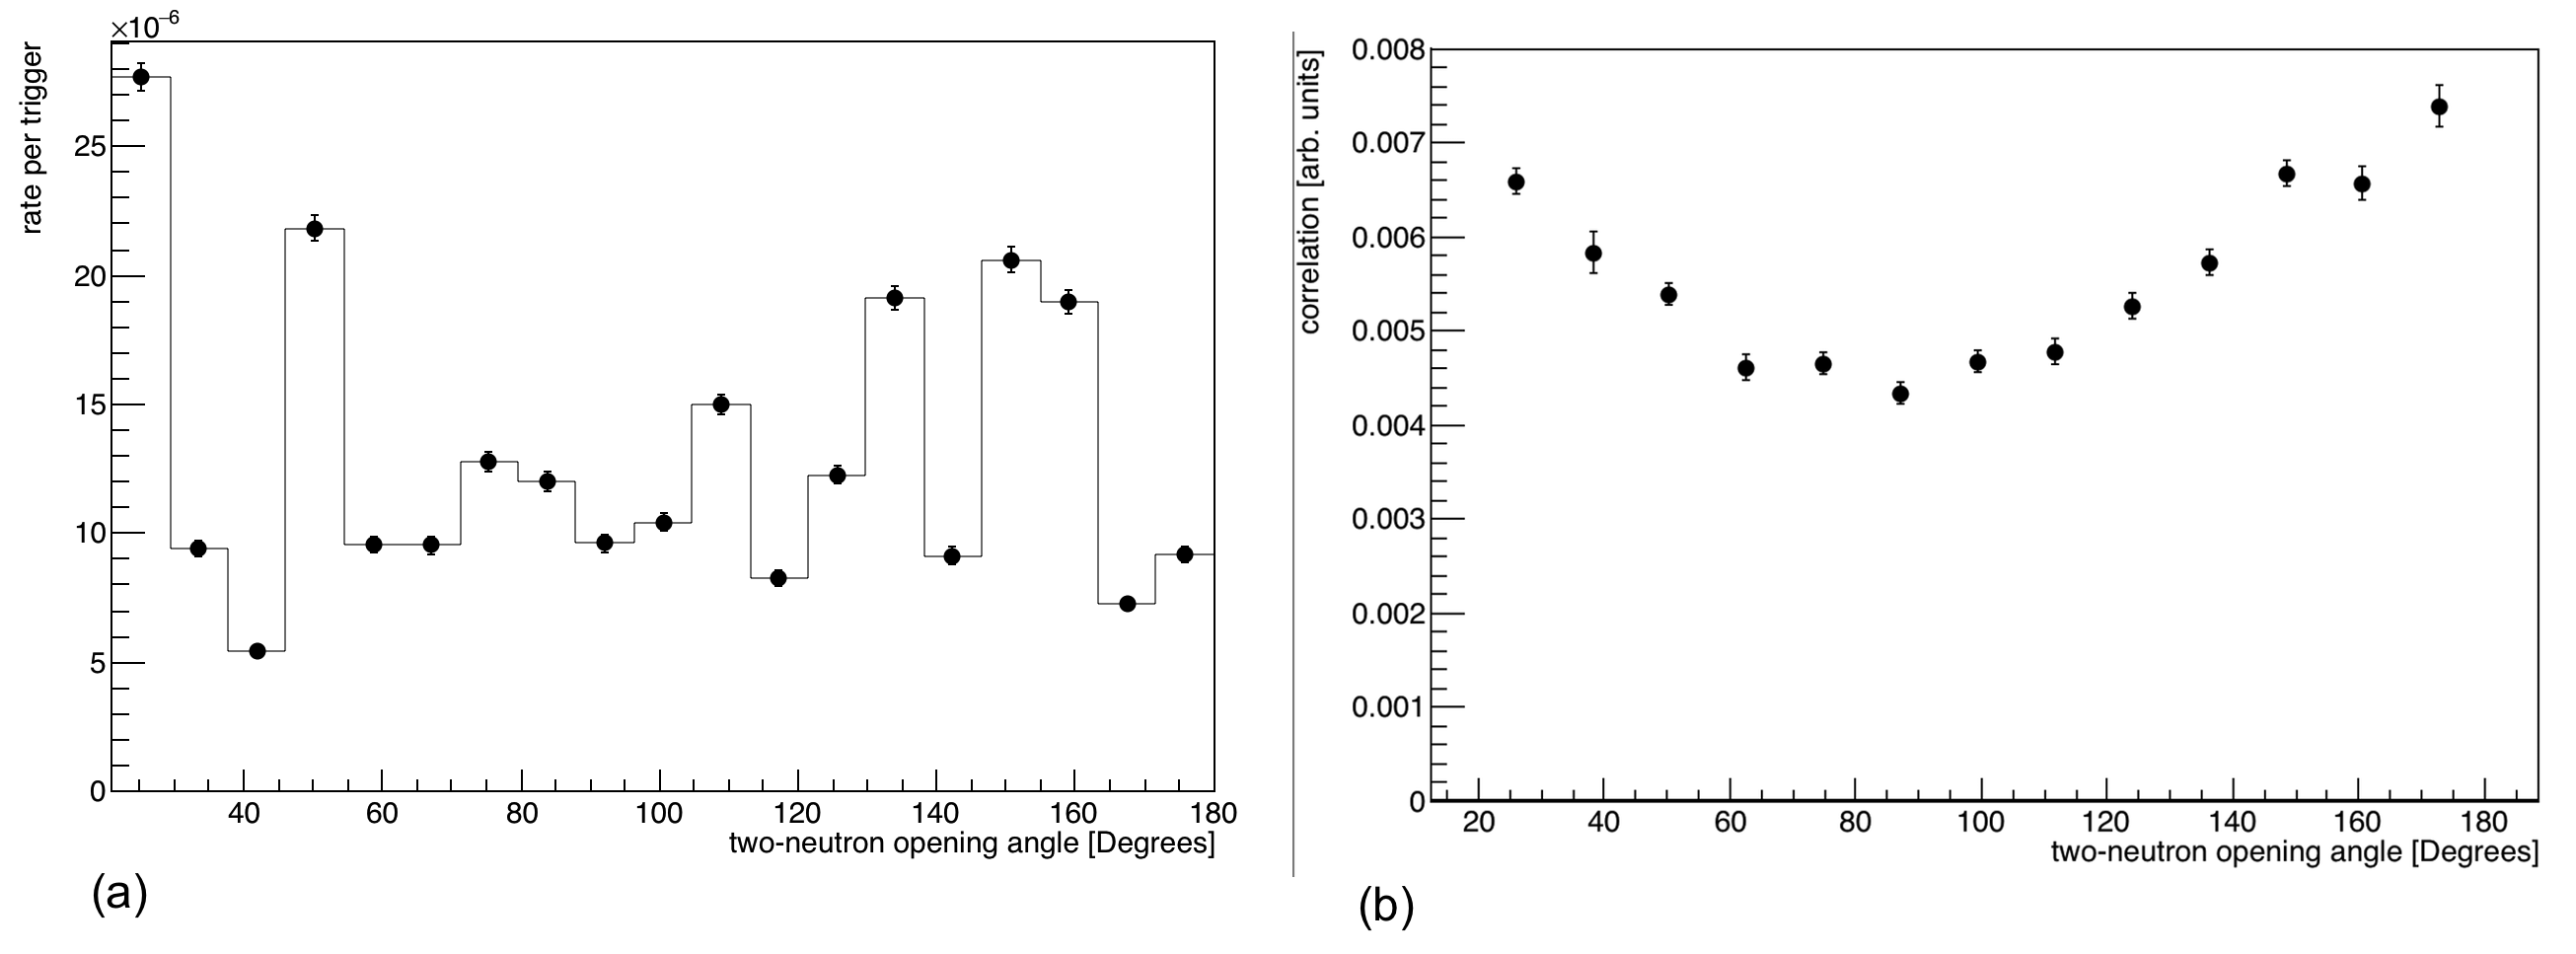
\includegraphics[width  = \textwidth ]{Content/Methods/Normalization.png}
    \caption{(a) Unnormalized two-neutron opening angle distribution from the spontaneous fission of $^{252}$Cf. The structure is reflective of geometric acceptance and efficiencies. (b) Same distribution after division by uncorrelated two-neutron events, which are taken from different pulses.}
    \label{fig:OpeningAngleAcceptance}
    \label{fig:OpeningAngleAcceptance}
\end{figure}
\subsection{Subtraction of Accidentals}
\label{Subtraction of Accidentals}
An accidental neutron coincidence is defined as a coincidence between two uncorrelated events in a single pulse.
For example, a coincidence between a neutron from a (gamma,1n) reaction and a neutron from photofission.
Another example is a coincidence between two events that are part of the noise background.
In both of these examples, the two events are considered accidentals because they have no causal influence on each another.
A true neutron coincidence, or true for short, is defined here as any pair correlated neutrons from the same pulse.

Accidentals are removed from the data by subtracting 1/2 times the equivalent distribution formed by the DP data.
The factor of 1/2 arises from the Poissonian statistics that inherently govern all accidentals, whether the accidental events are composed of two neutrons, two photons, two noise events, or any combination thereof.
% ToDo: Explain why the use of Poissonian statistics is valid.
An accidental is comprised of the occurrence of two independent events.
Therefore, as per Poissonian statistics, the probability of measuring an accidental in a single pulse is given by:
\begin{displaymath}
SP_{\text{a}} = \frac{e^{-\lambda}\lambda^2}{2} \approx \frac{1}{2}\lambda^{2}
\end{displaymath}
where $SP_{a}$ is the accidental rate of single pulses, $\lambda$ is the mean accidental rate of single pulses–an unknown value.
In this study, the coincidence rates were around $5\times10^{-5}$ events per pulse, so the approximation used above is correct to within 0.001\% as the worst case scenario.
Since the DP data is formed by observations of events from two different pulses, the DP accidental rate is equal to the Poissonian probability of one event, squared.
\begin{displaymath}
DP_{\text{a}} = (e^{-\lambda}\lambda)^{2}\approx \lambda^{2} 
\end{displaymath}
where $DP_{\text{a}}$ is the accidental rate of DP events.
Therefore, if coincidence rates, then the rate of measured accidentals in single pulses is 1/2 times the rate of accidentals in the different pulses.
In this study the subtraction had about a ten percent effect.



%%%%%% Errors %%%%%
\chapter{Discussion of Experimental Errors}
\label{Errors}
\thispagestyle{fancy}
\chapter{Discussion of Experimental Errors}
\label{Errors}
\section{Resolution of measurement}
The position of a detected particle is known to within a specified distance, which translates into a resolution in the measurement of the opening angle between a pair of particles.
A particle's reconstructed position along a detector's length has an error of $\pm$13 cm.
Due to the detector's 15 cm width, there is also a positional uncertainty of $\pm 7.5$ cm in the direction perpendicular to the detector's length.
The amount of uncertainty in a single two-neutron opening angle measurement is determined from of the uncertainties in the positions of each detected neutron.
These positional uncertainties are propagated through the formula for the calculation of opening angle, which is
\begin{displaymath}
    \theta_{nn} = \text{arccos}\left(\frac{\vec{v_{1}}^{\,}\cdot\vec{v_{2}}^{\,}}{|\vec{v_{1}}^{\,}||\vec{v_{2}}^{\,}|}\right)
\end{displaymath}
where $\vec{v_{1}}^{\,} = (x_1,y_1,z_1)$ and $\vec{v_{2}}^{\,} = (x_2,y_2,z_2)$ are the detected positions of the two neutrons.
The propagation of error through this formula is achieved by evaluating the following expression
\begin{eqnarray}
\label{eq:propagation}
 \Delta \theta_{nn} & = & \left( \left(\Delta x_1 \frac{\partial \theta}{\partial x_1}\right)^{2} + \left(\Delta y_1 \frac{\partial \theta}{\partial y_1}\right)^{2} + \left(\Delta z_1 \frac{\partial \theta}{\partial z_1}\right)^{2} + \right. \\
 & & \left. + \left(\Delta x_2 \frac{\partial \theta}{\partial x_2}\right)^{2} + \left(\Delta y_2\frac{\partial \theta}{\partial y_2}\right)^{2} + \left(\Delta z_2 \frac{\partial \theta}{\partial z_2}\right)^{2} \right) ^{\frac{1}{2}} \, ,  \nonumber
\end{eqnarray}
where the $\Delta$'s represent the uncertainty in the variable that directly follows each $\Delta$.
The values and uncertainties of all events in a given angle bin are fed through Eq.\ref{eq:propagation}, and then averaged together.
The result, seen in Fig.~\ref{fig:OpeningAngleRes}, can be interpreted as the opening angle resolution as a function of $\theta_{nn}$.
\begin{figure}[h]
    \centering
    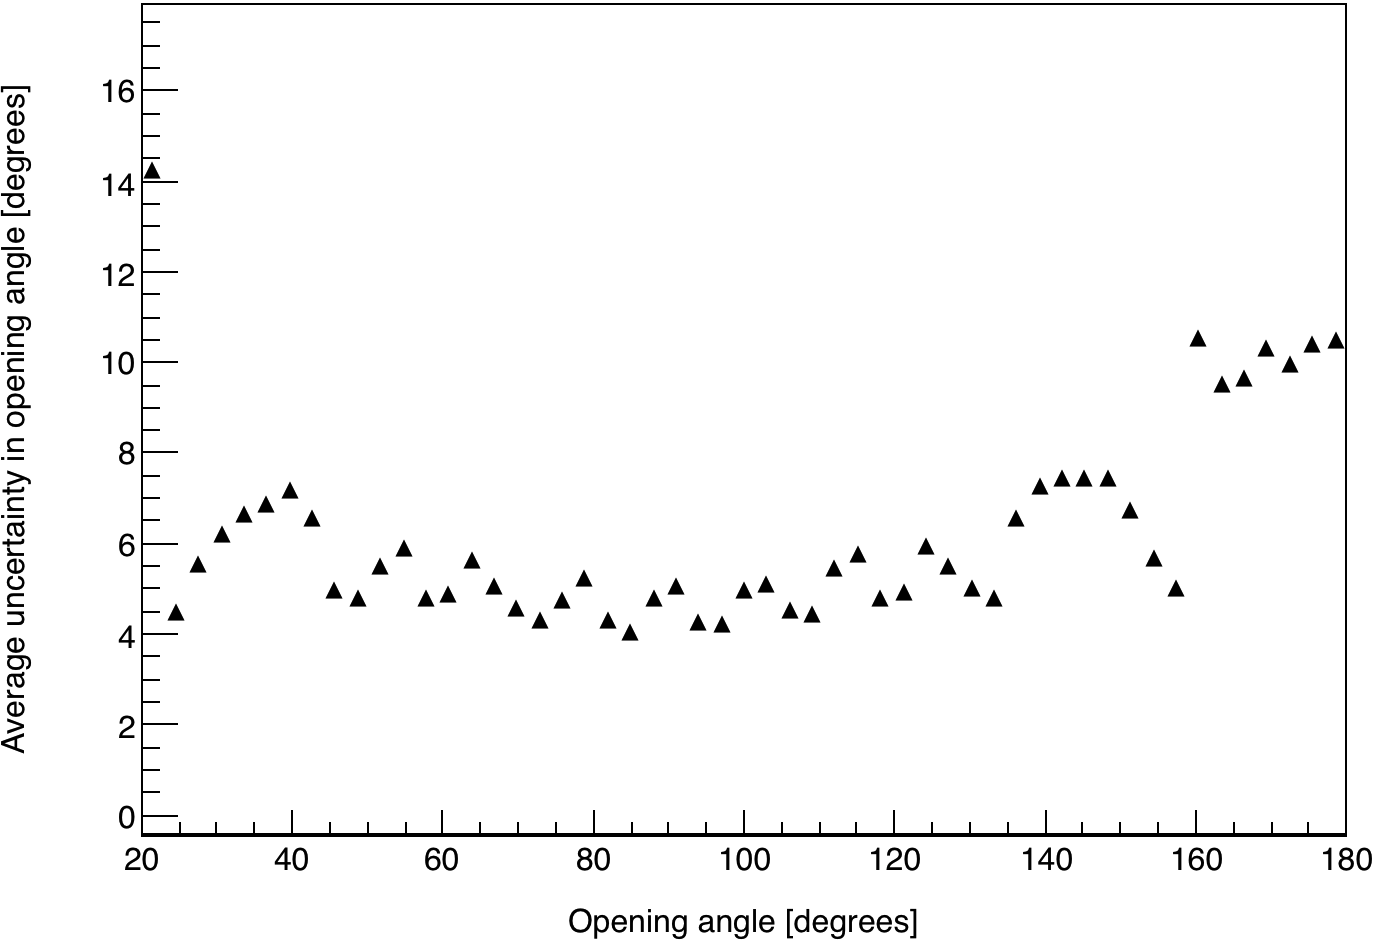
\includegraphics[width = 0.85\textwidth]{Content/Errors/OpeningAngleUncertainty.png}
    \caption{Uncertainties in opening angle determined from the propagation of position uncertainties through the opening angle calculation.
     The uncertainty of a given opening angle measurement depends on which detectors are involved and the position of the particles on the detectors.
     For this reason, the uncertainty of measurements falling within each angle bin is a distribution, so the average uncertainties are plotted here.
    The y-axis can be viewed as a measure of angular resolution in the sense that it represents the smallest angular difference that can be considered statistically significant.
    }
    \label{fig:OpeningAngleRes}
\end{figure}

\section{Counting error}
The uncertainty in the number of observed events is always assumed to be equal to $\sqrt{N}$, as per Poissonian  statistics, where N is the number of observed events.
This value is then propagated through all the analysis procedure using the standard methods for the propagation of error.
The vertical error bars seen in all results are due solely to such counting error.

\FloatBarrier
\section{Detector Cross-talk}
\label{crosstalk}
\textit{Cross-talk} occurs when, after a particle is detected once, the same particle, by any means, causes a detection to be registered in a different detector.
For example, upon detection, a particle may undergo elastic scattering and then travel into a another detector where it is detected again, or it may produce secondary particles that are detected.
The two coincident detections of a cross-talk event are causally correlated, and thus they have the potential to contaminate the signal from correlated fission neutrons.
If both detections occur during the ToF range typical for fission neutrons, then the cross-talk event cannot be distinguished from the detection of two correlated neutrons.

Recent works that measured the two-neutron angular correlations in the spontaneous fission of $^{252}$Cf and $^{240}$Pu~\cite{Pozzi2016,Verbeke2018} addressed this effect by using an MCNP-PoLiMi simulation to estimate and then subtract cross-talk from their measurements.
In this work, the issue of cross-talk is approached differently by employing the use of detector shielding aimed at reducing cross-talk to a negligible rate.
By using shielding to reduce cross-talk, this measurement is less dependent on the details of the models used by MCNP-PoLiMi to simulate neutron transport and detection.
MCNP-PoLoMi simulations are used in this work only to verify that the effect of cross-talk is negligible.
The scintillators used here are much larger than those used in similar works, such as in refs~\cite{Pozzi2016,Verbeke2018}, allowing for them to be placed much farther from the fission source without causing extremely low coincidence rates. 
An increase in the distance between the detectors and the fission source makes this measurement less sensitive to angular uncertainty, which is influenced by the uncertainty in the position of a detected particle due to, for example, the scattering of neutrons from detector shielding.
Because of this, larger amounts of shielding can be used without concern of introducing large errors.

The geometry of the neutron detection system makes it kinematically impossible for a neutron to scatter from a proton in one detector--which is the basis for scintillation--and then travel directly into another detector with enough kinetic energy to be detected a second time.
For this reason, upon being detected, a neutron must scatter from one or more intermediate nuclei, such as Pb or C, in order for it to reach a different detector with enough energy to be detected a second time.
This fact follows from the conservation of energy and momentum.
Figure~\ref{fig:CrossTalkExample} illustrates a cross-talk event due to a neutron scattering in a detector's shielding.
In order to be more convinced that such events occur at negligible rates, a detailed MCNP-PoliMi~\cite{MCNP_POLIMI} simulation was performed to model cross-talk.
\begin{figure}
    \centering
    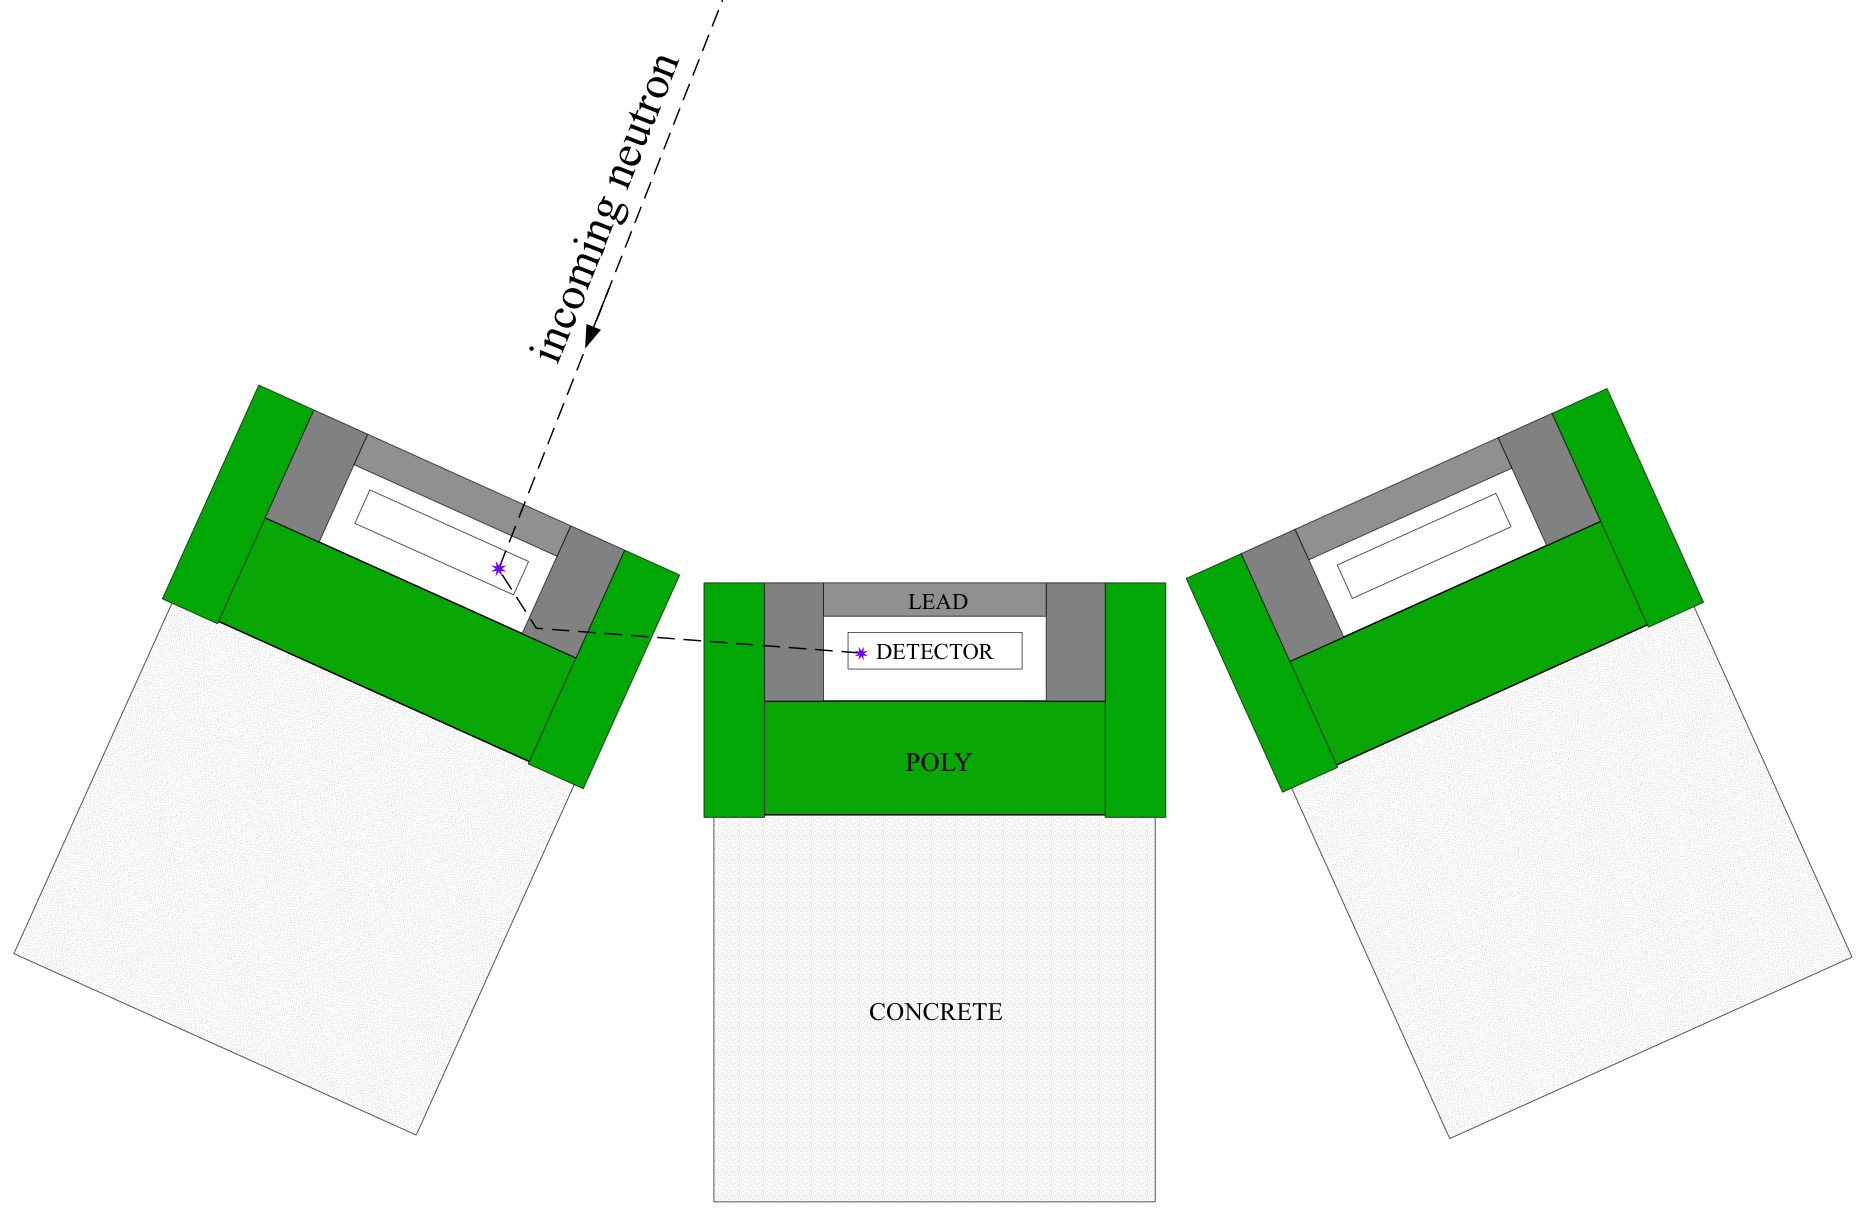
\includegraphics[width = 0.95\textwidth]{Content/Errors/CrossTalkExample.png}
    \caption{A hypothetical example of a neutron cross-talk event.
An incoming neutron is detected and then scatters from some lead shielding nearby, which changes its direction of travel such that it enters a second detector where it is detected a second time.
The scattering of a neutron from an intermediate nucleus, in this example a lead nucleus, is kinematically required in order for cross-talk to occur in this experiment.}
    \label{fig:CrossTalkExample}
\end{figure}

\section{Simulation of Detector Cross-talk}
A simulation was performed to ensure that the detector shielding effectively reduced cross-talk to negligible levels.
The simulation included all scintillators and their shielding, supporting structures, and the concrete walls surrounding the experimental cell.
MCNP-PoliMi's built-in $^{252}$Cf spontaneous fission source was used, which emits neutrons with the correct correlations and multiplicities.
Detector response was modeled using a program included with the MCNP-PoliMi distribution called MPPost~\cite{MPPost}.
The model is based on the electron equivalent light output (MeVee) produced by particles as they undergo collisions with carbon and hydrogen within organic plastic scintillators.
A minimum deposited energy of 0.4 MeV ( 0.05 MeVee for neutrons) was assumed for detectable particles, which was chosen because the neutron detection system showed a sharp decline in detection rates for neutrons below 0.4 MeV.
For neutron collisions with hydrogen, the light output in MeVee, $L$, is calculated by the following empirically derived formula
\begin{displaymath}
L = 0.0364 E_n^2 +  0.125 E_n
\end{displaymath}
where $E_n$ is equal to the loss in the kinetic energy of the neutron due to the collision.
Neutron interactions with carbon are assumed to generate a small light output of
\begin{displaymath}
L = 0.02 E_n
\end{displaymath}
As seen in Fig.~\ref{fig:Cf252MCNPVsEXP}, this model produces a ToF spectrum that is in good agreement with the measurement.
\begin{figure}
    \centering
    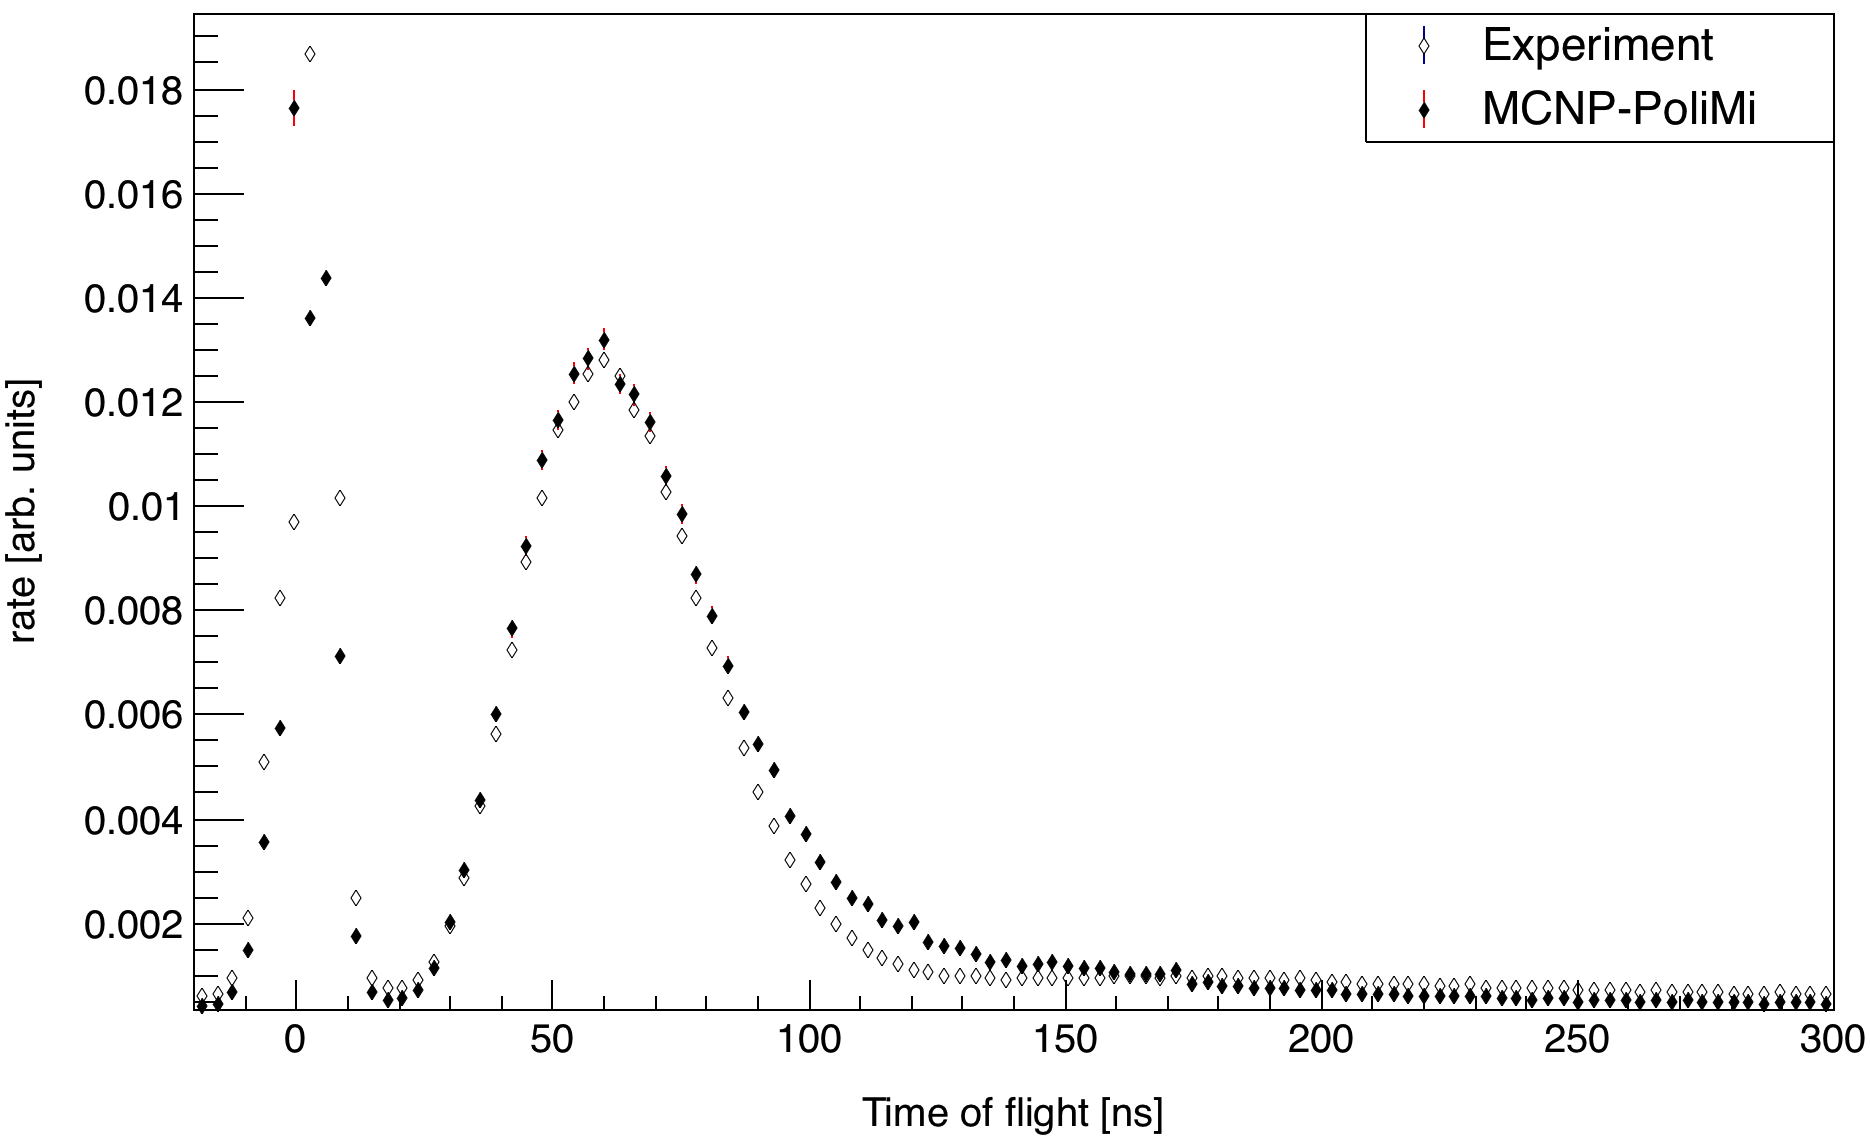
\includegraphics[width = 0.9\textwidth]{Content/Errors/Cf252MCNPVsEXP.png}
    \caption{Measured \emph{versus} simulated ToF spectrum of a $^{252}$Cf spontaneous fission source. 
    The simulation also used a detector response model based on ref~\cite{MPPost}}
    \label{fig:Cf252MCNPVsEXP}
\end{figure}

The simulation was initially performed with 5 cm of lead shielding placed behind the scintillators, and the number of cross-talk events accounted for 11\% of the total coincident neutron events.
The amount of cross-talk fell to 3\% if polyethylene was used instead of lead, which motivated the placement of 10~cm of polyethylene behind the detectors during construction.
Figure~\ref{fig:CrosstalkVScoincidence} shows the distribution of cross-talk events and true two-neutron coincidences as a function of reconstructed opening angle.
It is worth noting that, according to the simulation, the effect of cross-talk is not only small, but is also distributed over a wide range of angles rather than being concentrated around $\theta_{nn}=0$.
Angles greater than 125 degrees are not shown in Fig.~\ref{fig:CrosstalkVScoincidence}, because these cross-talk events can be readily identified in analysis by the large amount of time required for a neutron to travel the required distances.
\begin{figure}
    \centering
    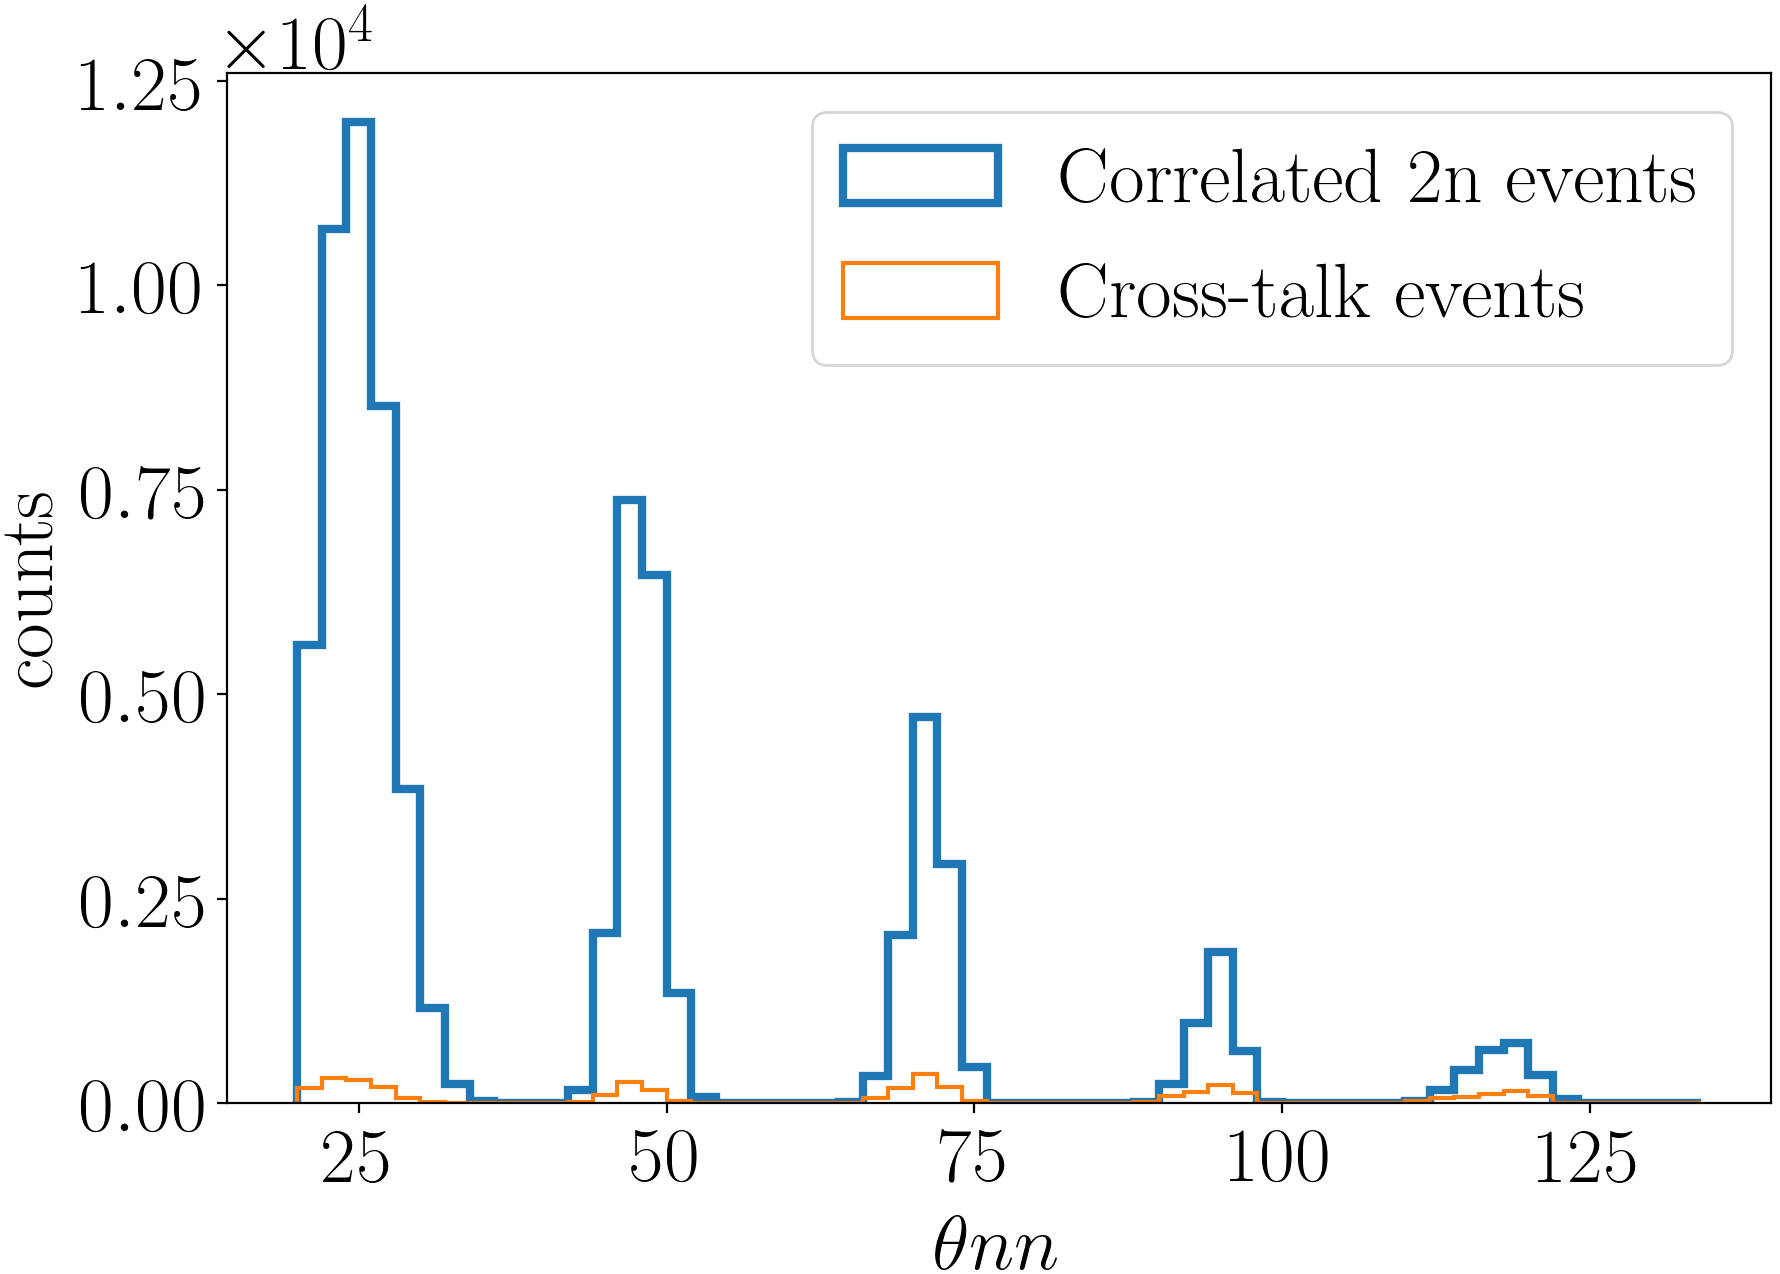
\includegraphics[width = 0.95\textwidth]{Content/Errors/CrosstalkVScoincidence.png}
    \caption{
    MCNP-PoLiMi simulation of the number of cross-talk events \emph{versus} correlated two-neutron events as a function of reconstructed opening angle.
    Cross-talk accounted for 3\% of total events.
    In this work, cross-talk does not occur primarily at small angles, but is instead spread out over a wide range of angles.
    }
    \label{fig:CrosstalkVScoincidence}
\end{figure}

\section{Neutron Scattering within Target}
\label{subsection:Elastic_scattering}
A potential source of error in opening angle measurements is the scattering of neutrons within the fission target.
This is a cause for concern, because a neutron that scatters from a heavy nucleons is very likely to be deflected at a large angle, creating two-neutron opening angles that are not reflective of the true opening angle immediately after fission.
Furthermore, because the target used in this work has the shape of a thin strip, it is more likely that neutrons that are initially traveling towards a given detector are deflected away by scattering if said detector is aligned along the wide (2~cm) axis of the strip, as opposed to the thin (0.05~cm) axis.
This bias is removed by slowly rotating the target about the vertical axis during data acquisition.
Because the subject of this measurement is fundamentally a statistical process, useful interpretations of the data are average rates taken over many events.
Thus, by rotating the target, cylindrical symmetry is preserved in the average, producing a result equivalent to that if a cylindrical target were used.

A thin strip is the ideal target shape regarding the rate of neutron elastic scattering per unit volume.
See Fig~\ref{fig:ElasticScatteringPlot} for the result of an MCNP simulation of the elastic scattering rates for both thin strip and cylindrical shaped targets.
The target in this experiment was a thin strip with a width 40 times greater than its thickness, for which the simulation indicated the rate of elastic scattering is roughly a factor of two less than for a cylindrical target of the same volume.

The target's dimensions are small enough that the rate of photon absorption, and thus photo-neutron production, is virtually uniform throughout the entire target volume.
MCNP was used to simulate the production of pairs of fission neutrons uniformly throughout the target volume with energies typical of fission neutrons.
The probability that at least one neutron out of a pair of two scatters before exiting the target was calculated from the simulation.
For the target used in this work, the simulation indicated that 6\% of two-neutron opening angles were altered due to scattering.
\begin{figure}
    \centering
    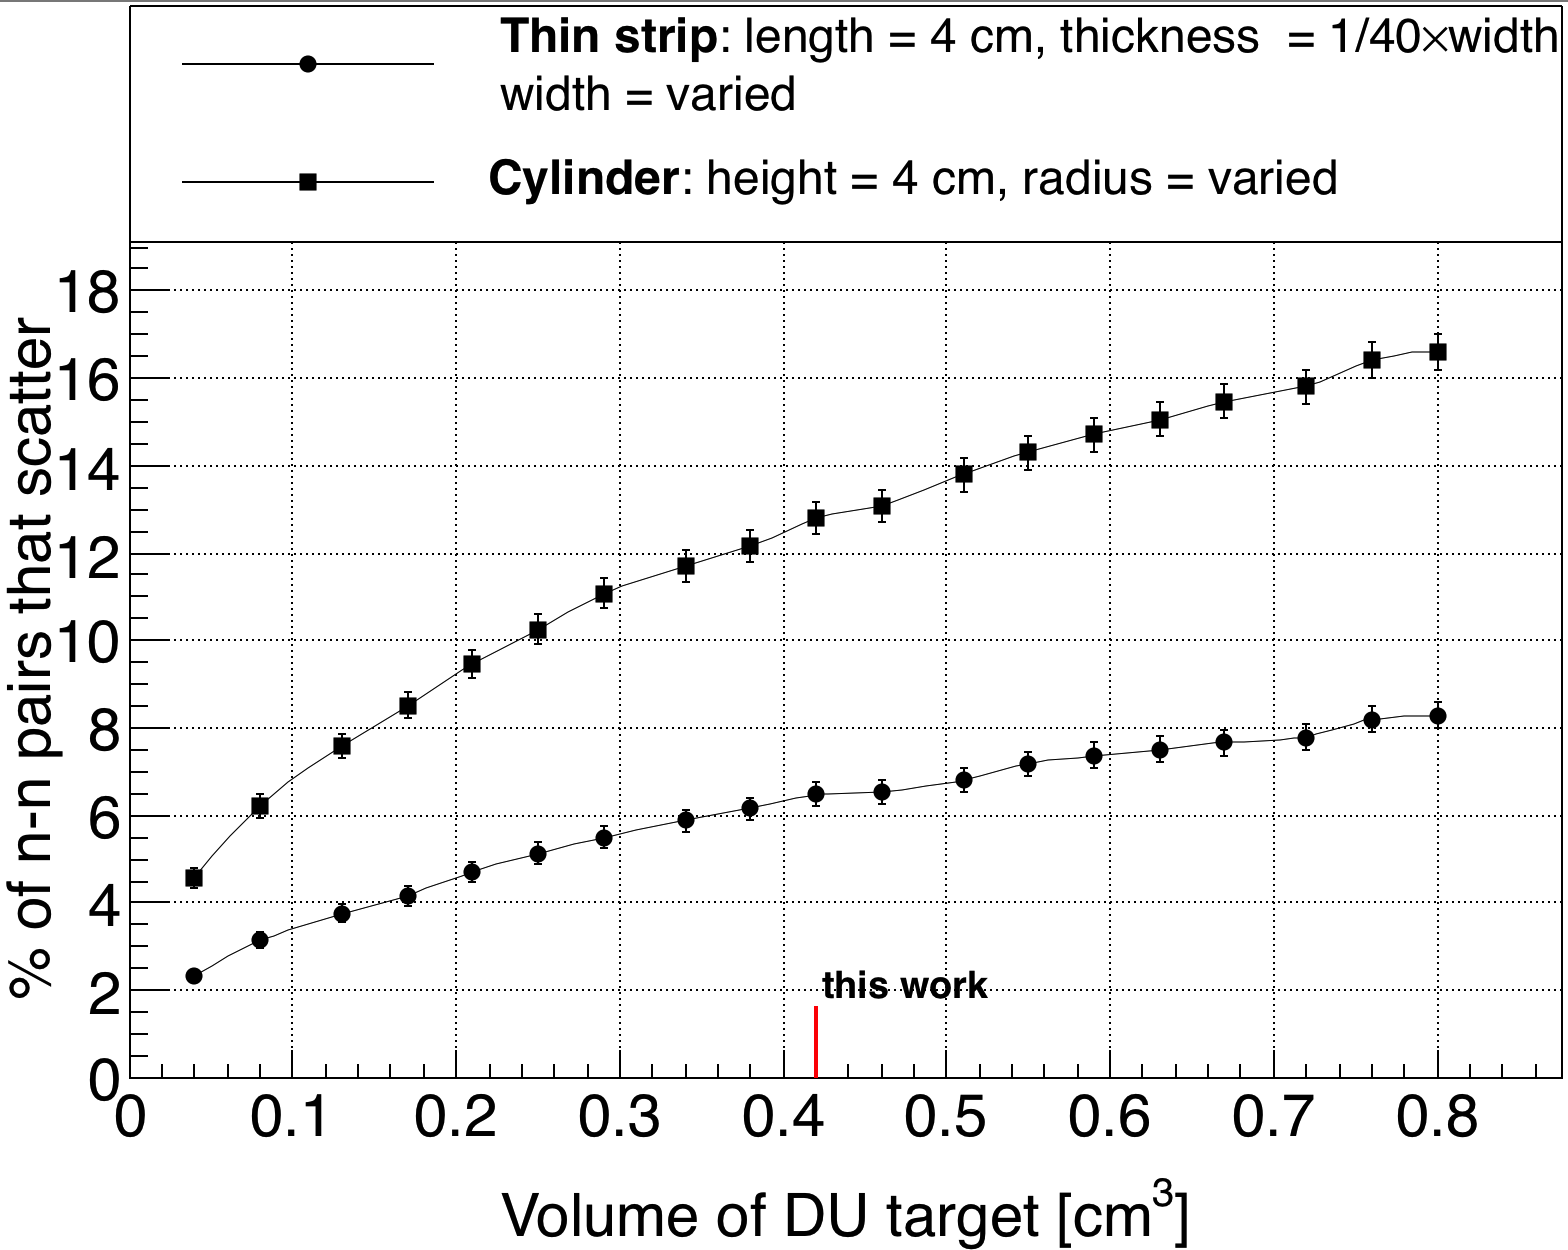
\includegraphics[width = 0.95\textwidth]{Content/Errors/ElasticScatteringPlot.png}
    \caption{
     Result of an MCNP simulation in which neutron-neutron pairs, with energies sampled from a typical watt fission spectrum, were generated uniformly throughout the volume of DU targets.
        The y-axis is the rate of opening angle contamination due to the scattering of, within the DU target in which they were produced, either one or both of a pair of neutrons.
    The lack of symmetry of a thin strip target can be removed by slowly rotating the target around the vertical axis during data acquisition, making it the optimal target geometry for the minimization of the rate of neutron scattering.
    The target used in this work had a length of 4~cm, a width of 2~cm, and a thickness of 0.05~cm.
    }
    \label{fig:ElasticScatteringPlot}
\end{figure}


\chapter{Discussion of Experimental Errors}
\label{Errors}
\section{Resolution of measurement}
The position of a detected particle is known to within a specified distance, which translates into a resolution in the measurement of the opening angle between a pair of particles.
A particle's reconstructed position along a detector's length has an error of $\pm$13 cm.
Due to the detector's 15 cm width, there is also a positional uncertainty of $\pm 7.5$ cm in the direction perpendicular to the detector's length.
The amount of uncertainty in a single two-neutron opening angle measurement is determined from of the uncertainties in the positions of each detected neutron.
These positional uncertainties are propagated through the formula for the calculation of opening angle, which is
\begin{displaymath}
    \theta_{nn} = \text{arccos}\left(\frac{\vec{v_{1}}^{\,}\cdot\vec{v_{2}}^{\,}}{|\vec{v_{1}}^{\,}||\vec{v_{2}}^{\,}|}\right)
\end{displaymath}
where $\vec{v_{1}}^{\,} = (x_1,y_1,z_1)$ and $\vec{v_{2}}^{\,} = (x_2,y_2,z_2)$ are the detected positions of the two neutrons.
The propagation of error through this formula is achieved by evaluating the following expression
\begin{eqnarray}
\label{eq:propagation}
 \Delta \theta_{nn} & = & \left( \left(\Delta x_1 \frac{\partial \theta}{\partial x_1}\right)^{2} + \left(\Delta y_1 \frac{\partial \theta}{\partial y_1}\right)^{2} + \left(\Delta z_1 \frac{\partial \theta}{\partial z_1}\right)^{2} + \right. \\
 & & \left. + \left(\Delta x_2 \frac{\partial \theta}{\partial x_2}\right)^{2} + \left(\Delta y_2\frac{\partial \theta}{\partial y_2}\right)^{2} + \left(\Delta z_2 \frac{\partial \theta}{\partial z_2}\right)^{2} \right) ^{\frac{1}{2}} \, ,  \nonumber
\end{eqnarray}
where the $\Delta$'s represent the uncertainty in the variable that directly follows each $\Delta$.
The values and uncertainties of all events in a given angle bin are fed through Eq.\ref{eq:propagation}, and then averaged together.
The result, seen in Fig.~\ref{fig:OpeningAngleRes}, can be interpreted as the opening angle resolution as a function of $\theta_{nn}$.
\begin{figure}[h]
    \centering
    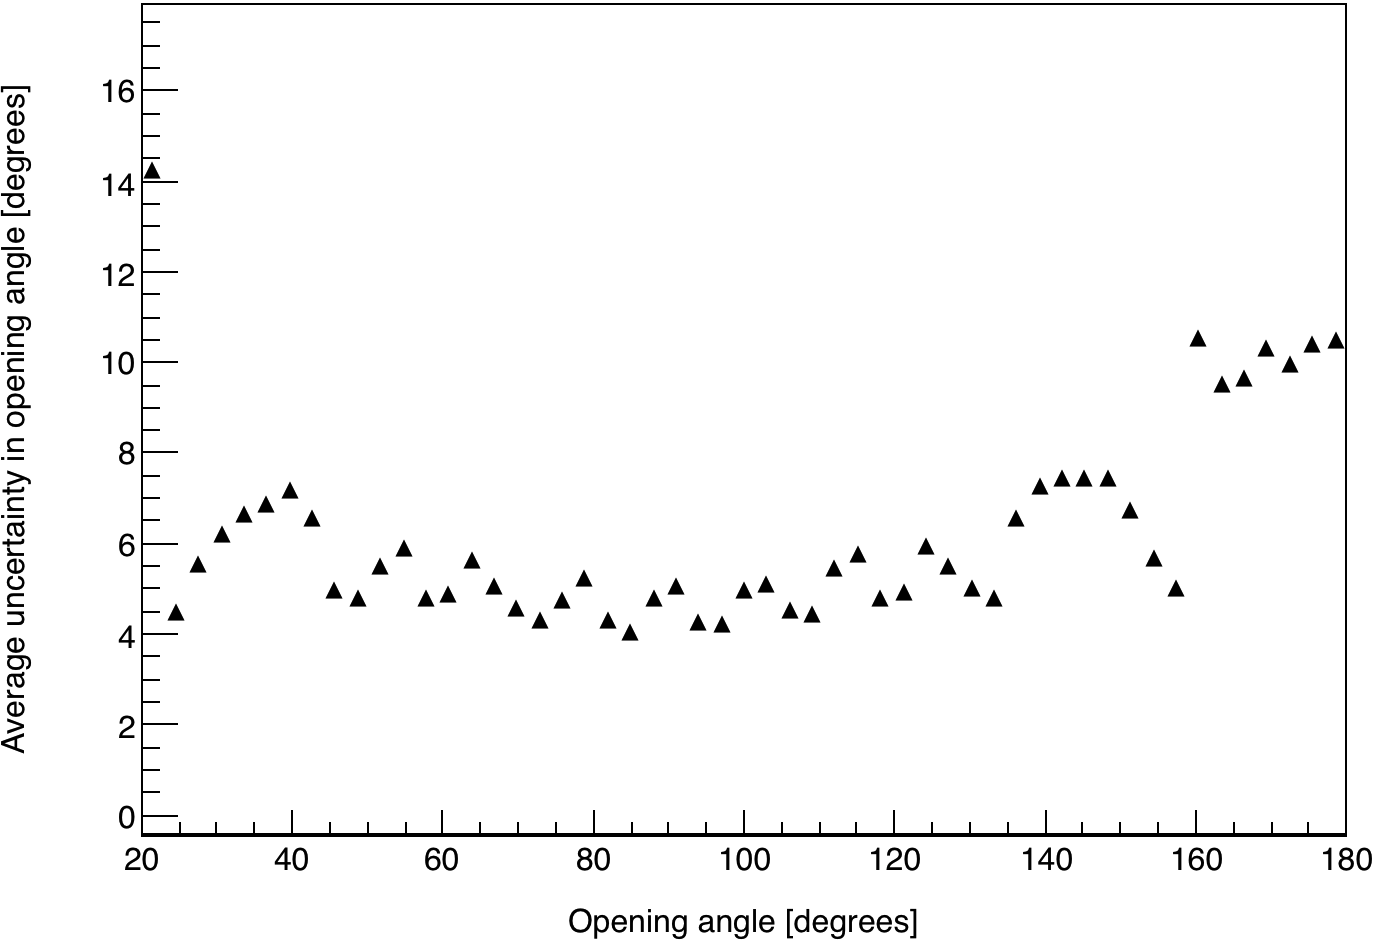
\includegraphics[width = 0.85\textwidth]{Content/Errors/OpeningAngleUncertainty.png}
    \caption{Uncertainties in opening angle determined from the propagation of position uncertainties through the opening angle calculation.
     The uncertainty of a given opening angle measurement depends on which detectors are involved and the position of the particles on the detectors.
     For this reason, the uncertainty of measurements falling within each angle bin is a distribution, so the average uncertainties are plotted here.
    The y-axis can be viewed as a measure of angular resolution in the sense that it represents the smallest angular difference that can be considered statistically significant.
    }
    \label{fig:OpeningAngleRes}
\end{figure}

\section{Counting error}
The uncertainty in the number of observed events is always assumed to be equal to $\sqrt{N}$, as per Poissonian  statistics, where N is the number of observed events.
This value is then propagated through all the analysis procedure using the standard methods for the propagation of error.
The vertical error bars seen in all results are due solely to such counting error.

\FloatBarrier
\section{Detector Cross-talk}
\label{crosstalk}
\textit{Cross-talk} occurs when, after a particle is detected once, the same particle, by any means, causes a detection to be registered in a different detector.
For example, upon detection, a particle may undergo elastic scattering and then travel into a another detector where it is detected again, or it may produce secondary particles that are detected.
The two coincident detections of a cross-talk event are causally correlated, and thus they have the potential to contaminate the signal from correlated fission neutrons.
If both detections occur during the ToF range typical for fission neutrons, then the cross-talk event cannot be distinguished from the detection of two correlated neutrons.

Recent works that measured the two-neutron angular correlations in the spontaneous fission of $^{252}$Cf and $^{240}$Pu~\cite{Pozzi2016,Verbeke2018} addressed this effect by using an MCNP-PoLiMi simulation to estimate and then subtract cross-talk from their measurements.
In this work, the issue of cross-talk is approached differently by employing the use of detector shielding aimed at reducing cross-talk to a negligible rate.
By using shielding to reduce cross-talk, this measurement is less dependent on the details of the models used by MCNP-PoLiMi to simulate neutron transport and detection.
MCNP-PoLoMi simulations are used in this work only to verify that the effect of cross-talk is negligible.
The scintillators used here are much larger than those used in similar works, such as in refs~\cite{Pozzi2016,Verbeke2018}, allowing for them to be placed much farther from the fission source without causing extremely low coincidence rates. 
An increase in the distance between the detectors and the fission source makes this measurement less sensitive to angular uncertainty, which is influenced by the uncertainty in the position of a detected particle due to, for example, the scattering of neutrons from detector shielding.
Because of this, larger amounts of shielding can be used without concern of introducing large errors.

The geometry of the neutron detection system makes it kinematically impossible for a neutron to scatter from a proton in one detector--which is the basis for scintillation--and then travel directly into another detector with enough kinetic energy to be detected a second time.
For this reason, upon being detected, a neutron must scatter from one or more intermediate nuclei, such as Pb or C, in order for it to reach a different detector with enough energy to be detected a second time.
This fact follows from the conservation of energy and momentum.
Figure~\ref{fig:CrossTalkExample} illustrates a cross-talk event due to a neutron scattering in a detector's shielding.
In order to be more convinced that such events occur at negligible rates, a detailed MCNP-PoliMi~\cite{MCNP_POLIMI} simulation was performed to model cross-talk.
\begin{figure}
    \centering
    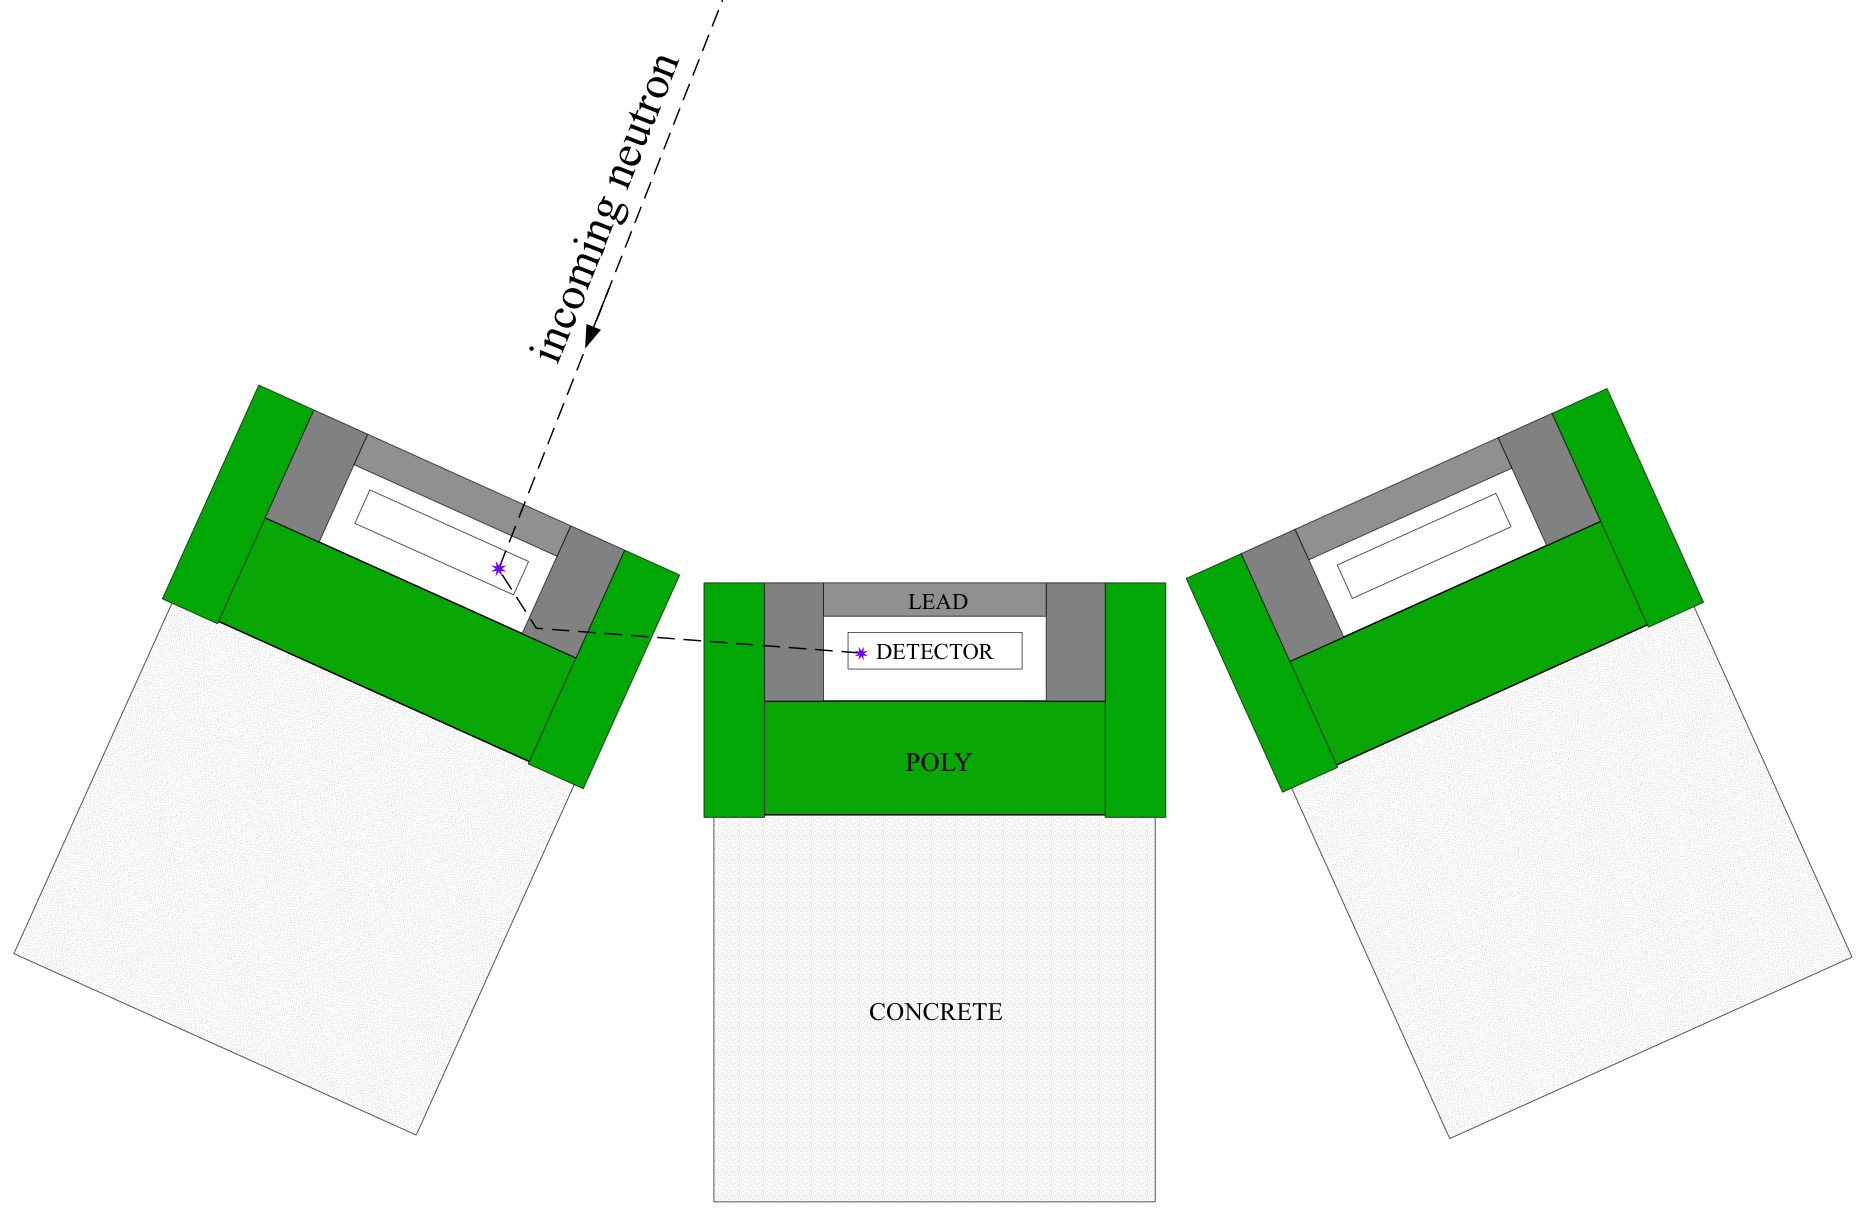
\includegraphics[width = 0.95\textwidth]{Content/Errors/CrossTalkExample.png}
    \caption{A hypothetical example of a neutron cross-talk event.
An incoming neutron is detected and then scatters from some lead shielding nearby, which changes its direction of travel such that it enters a second detector where it is detected a second time.
The scattering of a neutron from an intermediate nucleus, in this example a lead nucleus, is kinematically required in order for cross-talk to occur in this experiment.}
    \label{fig:CrossTalkExample}
\end{figure}

\section{Simulation of Detector Cross-talk}
A simulation was performed to ensure that the detector shielding effectively reduced cross-talk to negligible levels.
The simulation included all scintillators and their shielding, supporting structures, and the concrete walls surrounding the experimental cell.
MCNP-PoliMi's built-in $^{252}$Cf spontaneous fission source was used, which emits neutrons with the correct correlations and multiplicities.
Detector response was modeled using a program included with the MCNP-PoliMi distribution called MPPost~\cite{MPPost}.
The model is based on the electron equivalent light output (MeVee) produced by particles as they undergo collisions with carbon and hydrogen within organic plastic scintillators.
A minimum deposited energy of 0.4 MeV ( 0.05 MeVee for neutrons) was assumed for detectable particles, which was chosen because the neutron detection system showed a sharp decline in detection rates for neutrons below 0.4 MeV.
For neutron collisions with hydrogen, the light output in MeVee, $L$, is calculated by the following empirically derived formula
\begin{displaymath}
L = 0.0364 E_n^2 +  0.125 E_n
\end{displaymath}
where $E_n$ is equal to the loss in the kinetic energy of the neutron due to the collision.
Neutron interactions with carbon are assumed to generate a small light output of
\begin{displaymath}
L = 0.02 E_n
\end{displaymath}
As seen in Fig.~\ref{fig:Cf252MCNPVsEXP}, this model produces a ToF spectrum that is in good agreement with the measurement.
\begin{figure}
    \centering
    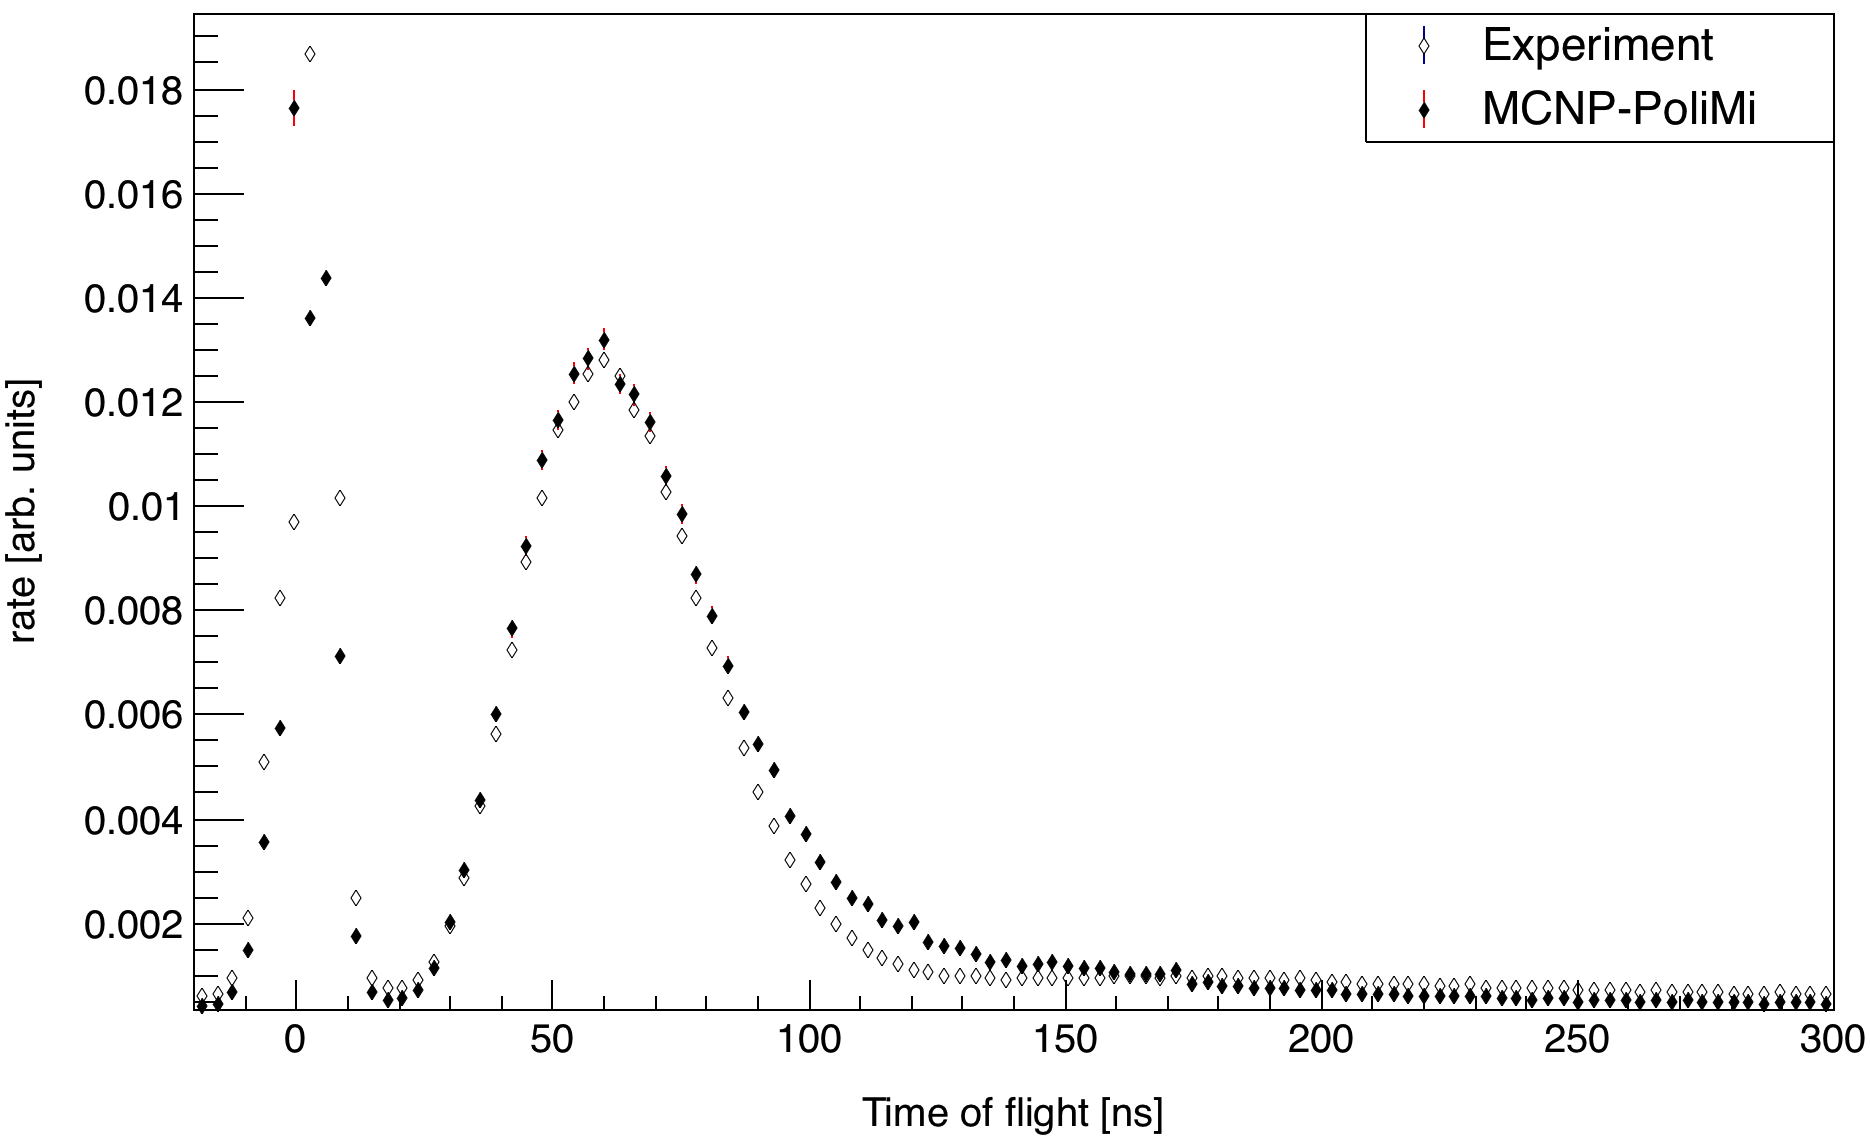
\includegraphics[width = 0.9\textwidth]{Content/Errors/Cf252MCNPVsEXP.png}
    \caption{Measured \emph{versus} simulated ToF spectrum of a $^{252}$Cf spontaneous fission source. 
    The simulation also used a detector response model based on ref~\cite{MPPost}}
    \label{fig:Cf252MCNPVsEXP}
\end{figure}

The simulation was initially performed with 5 cm of lead shielding placed behind the scintillators, and the number of cross-talk events accounted for 11\% of the total coincident neutron events.
The amount of cross-talk fell to 3\% if polyethylene was used instead of lead, which motivated the placement of 10~cm of polyethylene behind the detectors during construction.
Figure~\ref{fig:CrosstalkVScoincidence} shows the distribution of cross-talk events and true two-neutron coincidences as a function of reconstructed opening angle.
It is worth noting that, according to the simulation, the effect of cross-talk is not only small, but is also distributed over a wide range of angles rather than being concentrated around $\theta_{nn}=0$.
Angles greater than 125 degrees are not shown in Fig.~\ref{fig:CrosstalkVScoincidence}, because these cross-talk events can be readily identified in analysis by the large amount of time required for a neutron to travel the required distances.
\begin{figure}
    \centering
    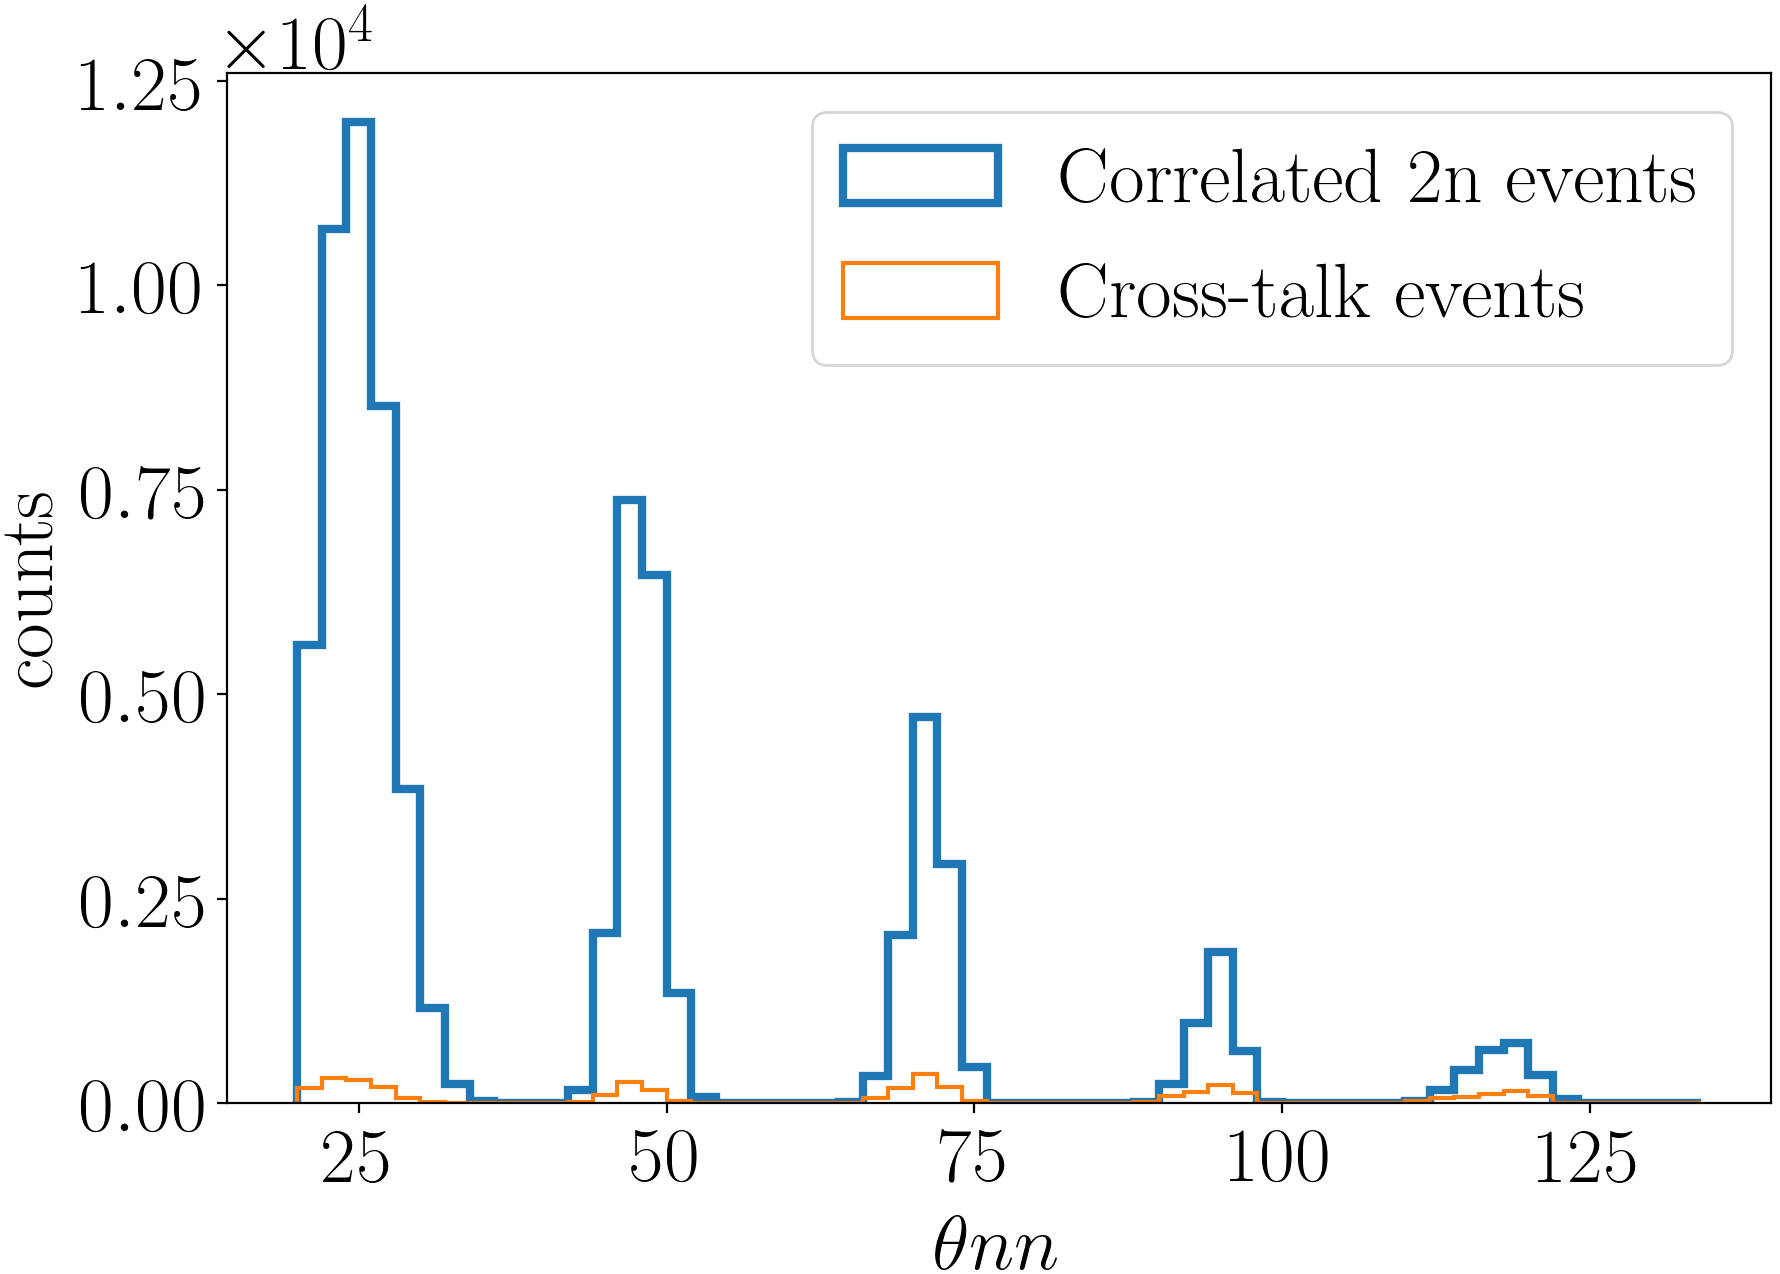
\includegraphics[width = 0.95\textwidth]{Content/Errors/CrosstalkVScoincidence.png}
    \caption{
    MCNP-PoLiMi simulation of the number of cross-talk events \emph{versus} correlated two-neutron events as a function of reconstructed opening angle.
    Cross-talk accounted for 3\% of total events.
    In this work, cross-talk does not occur primarily at small angles, but is instead spread out over a wide range of angles.
    }
    \label{fig:CrosstalkVScoincidence}
\end{figure}

\section{Neutron Scattering within Target}
\label{subsection:Elastic_scattering}
A potential source of error in opening angle measurements is the scattering of neutrons within the fission target.
This is a cause for concern, because a neutron that scatters from a heavy nucleons is very likely to be deflected at a large angle, creating two-neutron opening angles that are not reflective of the true opening angle immediately after fission.
Furthermore, because the target used in this work has the shape of a thin strip, it is more likely that neutrons that are initially traveling towards a given detector are deflected away by scattering if said detector is aligned along the wide (2~cm) axis of the strip, as opposed to the thin (0.05~cm) axis.
This bias is removed by slowly rotating the target about the vertical axis during data acquisition.
Because the subject of this measurement is fundamentally a statistical process, useful interpretations of the data are average rates taken over many events.
Thus, by rotating the target, cylindrical symmetry is preserved in the average, producing a result equivalent to that if a cylindrical target were used.

A thin strip is the ideal target shape regarding the rate of neutron elastic scattering per unit volume.
See Fig~\ref{fig:ElasticScatteringPlot} for the result of an MCNP simulation of the elastic scattering rates for both thin strip and cylindrical shaped targets.
The target in this experiment was a thin strip with a width 40 times greater than its thickness, for which the simulation indicated the rate of elastic scattering is roughly a factor of two less than for a cylindrical target of the same volume.

The target's dimensions are small enough that the rate of photon absorption, and thus photo-neutron production, is virtually uniform throughout the entire target volume.
MCNP was used to simulate the production of pairs of fission neutrons uniformly throughout the target volume with energies typical of fission neutrons.
The probability that at least one neutron out of a pair of two scatters before exiting the target was calculated from the simulation.
For the target used in this work, the simulation indicated that 6\% of two-neutron opening angles were altered due to scattering.
\begin{figure}
    \centering
    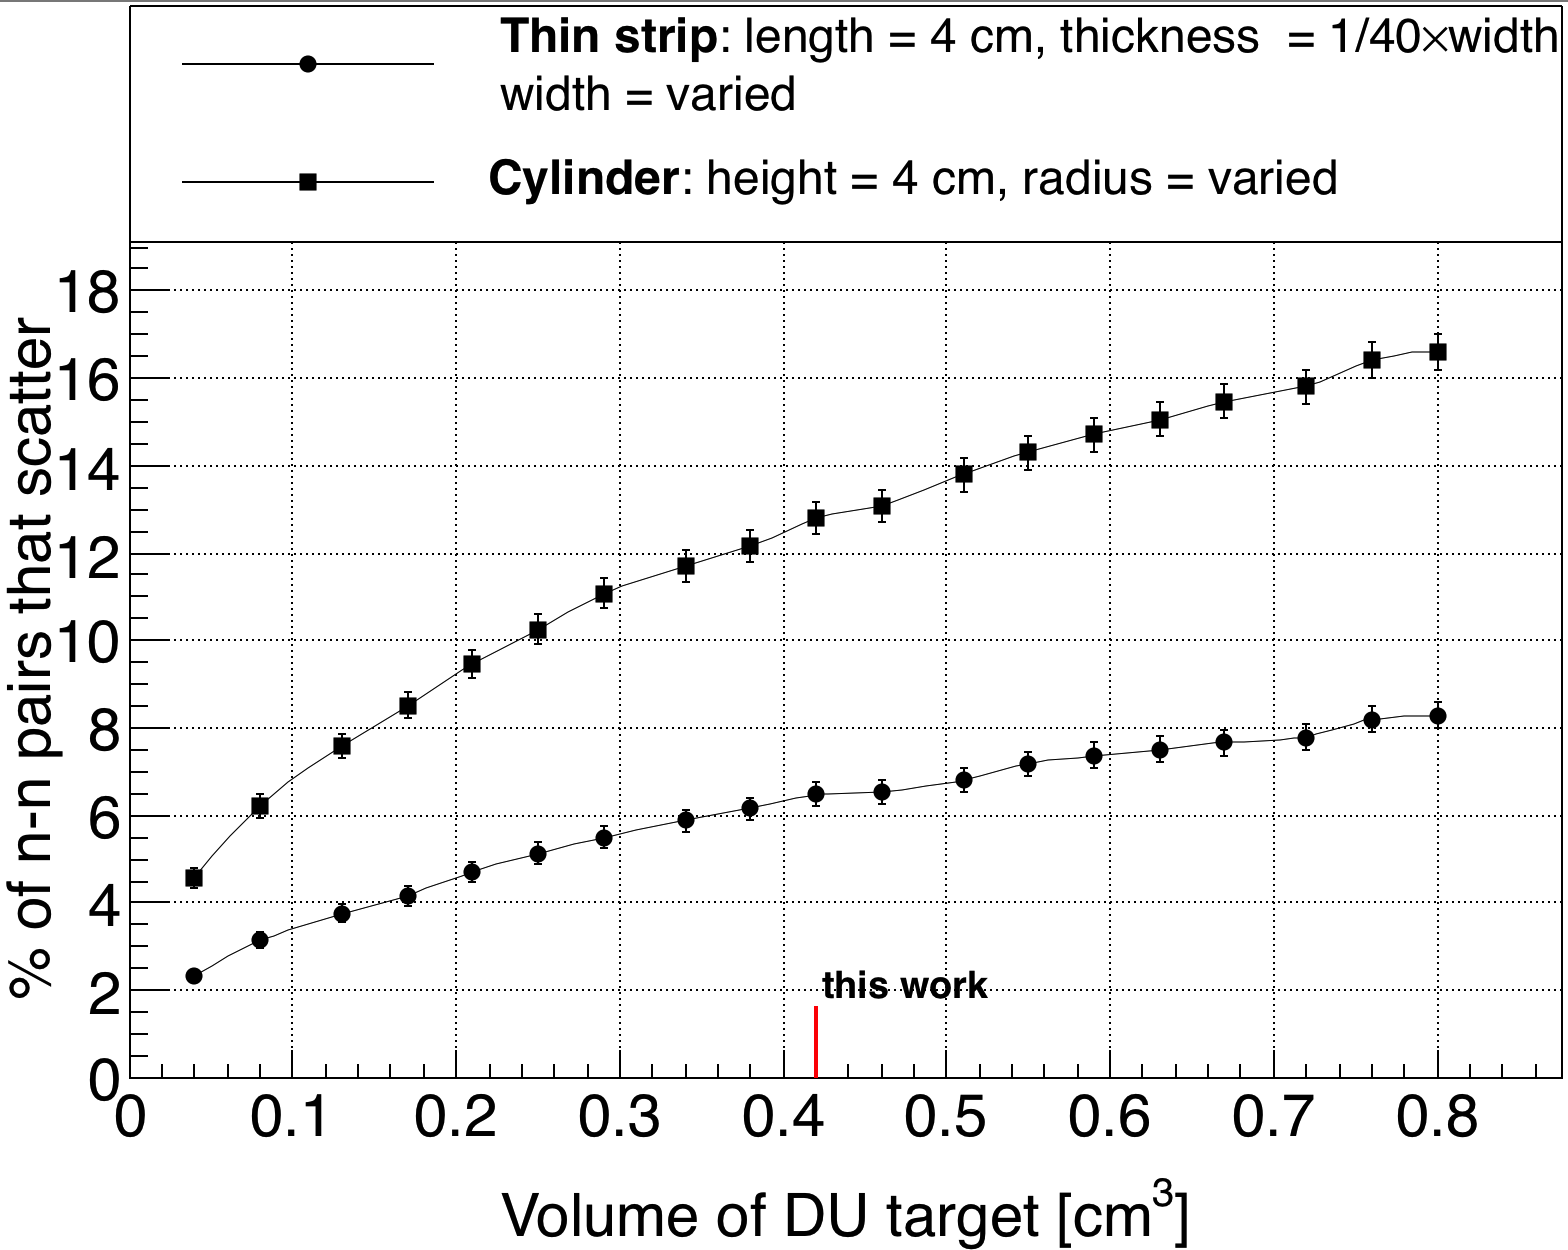
\includegraphics[width = 0.95\textwidth]{Content/Errors/ElasticScatteringPlot.png}
    \caption{
     Result of an MCNP simulation in which neutron-neutron pairs, with energies sampled from a typical watt fission spectrum, were generated uniformly throughout the volume of DU targets.
        The y-axis is the rate of opening angle contamination due to the scattering of, within the DU target in which they were produced, either one or both of a pair of neutrons.
    The lack of symmetry of a thin strip target can be removed by slowly rotating the target around the vertical axis during data acquisition, making it the optimal target geometry for the minimization of the rate of neutron scattering.
    The target used in this work had a length of 4~cm, a width of 2~cm, and a thickness of 0.05~cm.
    }
    \label{fig:ElasticScatteringPlot}
\end{figure}


\section{Neutron Scattering within Target}
\input{../nnCorrPhysRev/Elastic_Scat_in_target.tex}

%%%%%% Results %%%%%
\chapter{Results}


%%%%%% Conclusion %%%%%
\chapter{Concluding Remarks}
\thispagestyle{fancy}
\input{../nnCorrPhysRev/Conclude.tex}


%backmatter
\thispagestyle{fancy}
\bibliography{../nnCorrPhysRev/refs.bib}


\chapter{Appendix}
\thispagestyle{fancy}
\section{Rates}
\label{sec:rates}
Table~\ref{table:rates} shows the rates, per pulse, of the detection of photons and neutrons for each detector.
The overall rate of neutron singles and doubles was 4.89$\times 10^{-3}$ and 3.57$\times 10^{-5}$ per pulse, respectively.
\begin{center}
 \begin{table}
 \centering
\begin{tabular}{c  S[table-format=1.4e-2] S[table-format=1.4e-2]}%S[table-format=1.4]} %{||c |c |c |c| c||}  ccS[table-format=1.4e-2]
 \toprule
\textbf{Detector} & \textbf{neutron rate} & \textbf{photon rate} \\ [0.5ex] 
\midrule
30 bottom & 4.43E-04 & 1.93E-01 \\ \midrule
30 top & 2.11E-04 & 1.68E-01 \\ \midrule
54 & 5.03E-04 & 3.77E-01 \\ \midrule
78 & 4.27E-04 & 9.67E-02 \\ \midrule
102 & 3.61E-04 & 4.73E-02 \\ \midrule
126 & 7.13E-04 & 5.14E-02 \\ \midrule
150 & 5.76E-04 & 3.79E-02 \\ \midrule
210 & 7.16E-04 & 4.99E-02 \\ \midrule
234 & 4.49E-04 & 4.49E-02 \\ \midrule
258 & 5.27E-04 & 5.90E-02 \\ \midrule
282 & 4.42E-04 & 1.04E-01 \\ \midrule
306 & 3.40E-04 & 3.17E-01 \\ \midrule
330 bottom & 3.46E-04 & 2.35E-01 \\ \midrule
330 top & 3.24E-04 & 2.50E-01 \\
\bottomrule
\end{tabular}
\caption{
Per pulse rate of neutrons and photons on each detector.
Only one particle can be detected by a given detector per pulse, so the rate of photon detection affects the measured neutron rate.
}
  \label{table:rates}
\end{table}
\end{center}


\end{document}